\vspace{0.015\textheight}
This study is performed at the world's highest energy proton-antiproton collider, the Tevatron, which operates at the Fermi National Accelerator Laboratory (Fermilab) located just west of the city of Chicago. The 4-mile-long accelerator ring accelerates protons and antiprotons close to the speed of light and collides them in order to unravel mysteries of the subatomic world. An overview of the Tevatron accelerator and the Collider Detector at Fermilab (CDF) experiment, where the data are collected, is described in this chapter. Different subdetectors of the CDF detector are described together with their purpose for this analysis. In addition, some of the contributions of the author to the operation of the CDF detector subsystems is described. Finally, the method of extracting interesting physics events from hadron collisions is explained.

\section{The Tevatron}

\begin{figure}[htb!]
\begin{centering}
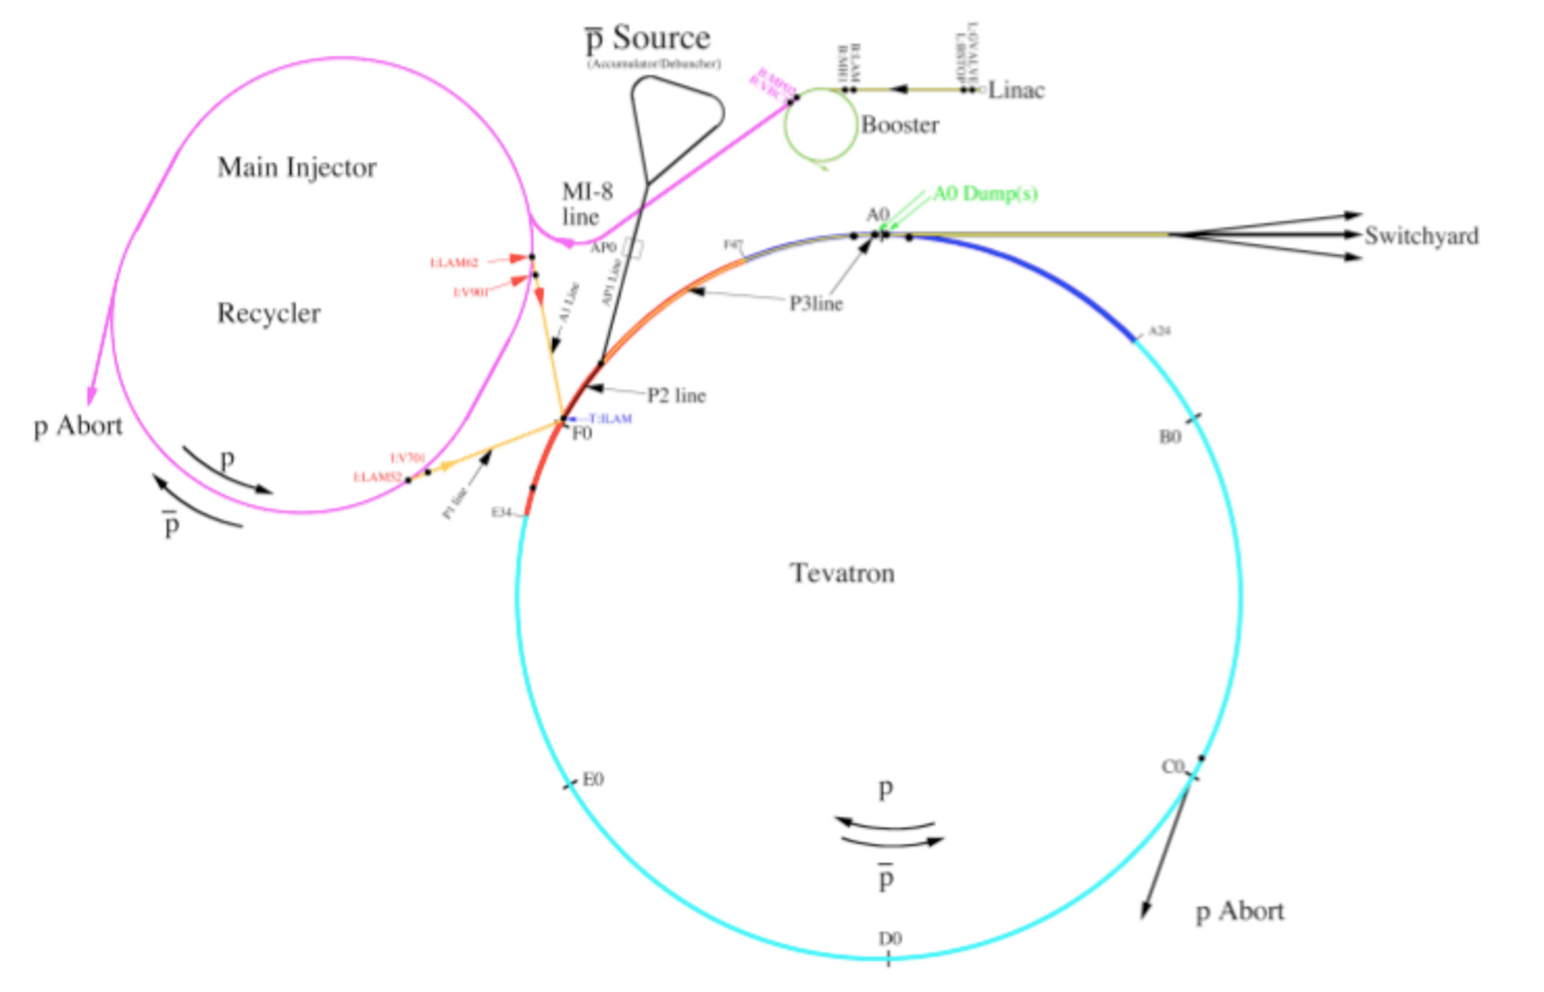
\includegraphics[scale=0.6]{AcceleratorOverview.pdf}
\caption{Overview of the accelerator complex.}
\label{fig_AcceleratorOverview}
\end{centering}
\end{figure}

The Tevatron is the largest of the Fermilab accelerators (see Fig.~\ref{fig_AcceleratorOverview}). It is a synchrotron (circular accelerator) where two particle beams, protons ($p$) and antiprotons ($\bar{p}$), circulate in opposite directions. With its eight accelerating cavities, it can accelerate protons and antiprotons up to \mbox{980 GeV}, yielding a center of mass energy ($\sqrt{s}$) of \mbox{1.96 TeV}. A large number of superconducting magnets placed along the beam pipe steer the beam around the ring. An extensive cryogenic cooling system keeps these superconducting magnets at subzero temperatures (\mbox{$\sim$4 K}). Because the magnets are superconducting, a large magnetic field can be achieved with only one-third of the power of regular magnet. The accelerated beams are collided at two points located around the the ring, at the center of the CDF and D\O~detectors.

\subsection{Pre-accelerator}
The acceleration process starts when protons are extracted from hydrogen gas in the pre-accelerator or Preacc. The Preacc houses a proton source that converts hydrogen gas to ionized hydrogen gas ($H^{-}$) that is accelerated to an energy of \mbox{750 keV} using an electrostatic potential difference. At this initial stage the Preacc accelerates the beam every \mbox{66 ms}, or at a rate of \mbox{15 Hz}. Then the beam is transfered to the next level of acceleration, the Linac.

\subsection{Linac}
The Linac is a linear accelerator that accelerates the hydrogen ions to \mbox{400 MeV} using a combination of drift tubes and radio frequency (RF) cavities. The Linac operates at the same frequency as the Preacc. Several quadrupole magnets placed inside the drift tubes, along the accelerating modules, focus the beam before handing it over to the Booster.

\subsection{Booster}
The Booster, with a \mbox{75 m} radius, is the first synchrotron in the chain of accelerators. A series of magnets are arranged around the ring, intermixed with 18 RF cavities. The Booster first strips off the electrons from the 400~MeV hydrogen ions to make protons and then it accelerates the protons to \mbox{8 GeV} of energy. The Booster operates at \mbox{15 Hz} and can accelerate the beam once every 66 milliseconds. From the Booster, the beam goes to the Main Injector.

\subsection{Main Injector}
The Main Injector (MI) is the second synchrotron in the chain with a size just over half the circumference of the Tevatron. In addition to accepting protons from the Booster, the MI also accepts antiprotons from the antiproton source. Using its 18 acceleration cavities, the MI accelerates protons from the Booster up to \mbox{150 GeV}. If it is used to accumulate antiprotons, it will accelerate them to \mbox{120 GeV}. When used to inject proton and anitprotons beams into the Tevatron, it will accelerate the beams to \mbox{150 GeV}. The MI also delivers particle beams with different energies to other experiments on site.

\subsection{Antiproton Generation}
Antiprotons are produced by firing protons into a fixed target. One batch of protons from the Booster is injected into the Main Injector and accelerated to \mbox{120 GeV}. This proton beam is fired into a fixed nickel target. Upon impact, these high-energy protons produce a whole collection of secondary particles. Magnets are tuned to collect 8~GeV antiprotons from this spray as illustrated in Fig.~\ref{fig:AntiProtonProduction}. It takes less than a day to produce enough antiprotons for collisions in the Tevatron.

\begin{figure}[htbm]
 \centering
 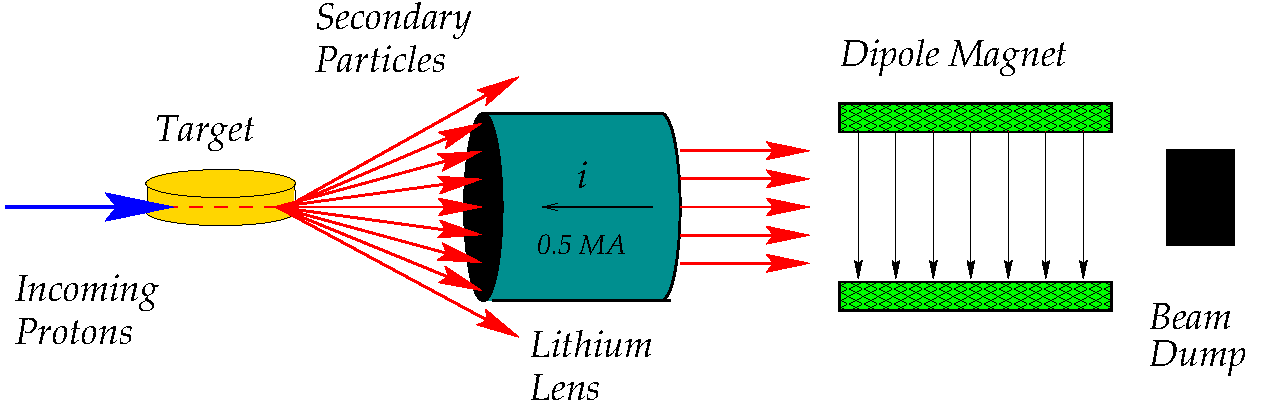
\includegraphics[scale=0.7,keepaspectratio=true,angle=0]{./Antiproton_production.pdf}
 % Antiproton_production.pdf: 255x779 pixel, 72dpi, 9.00x27.48 cm, bb=0 0 255 779
 \caption{Illustration of antiproton production. The dipole magnet directs the antiprotons to the Debuncher and other particles are sent to the beam dump.}
 \label{fig:AntiProtonProduction}
\end{figure}
\vspace{-0.03\textheight}

\subsection{Debuncher}
The Debuncher is a rounded-triangular synchrotron, and its primary purpose is to efficiently capture the antiprotons coming off the target, which have a very high momentum spread. The Debuncher does not accelerate the beam, but instead it helps to reduce the momentum spread. To accomplish this goal, it is equipped with a stochastic cooling system. In stochastic cooling, a signal is picked up from the circulating antiprotons at one side of the ring. That signal is amplified and sent directly across the ring. There, it is used to affect the trajectories of the antiprotons when they arrive. The Debuncher transfers the beam to the Accumulator, which holds the cooled antiprotons at 8~GeV until needed.

\subsection{Structure of Colliding Beams}
The Tevatron collides beams of protons and antiprotons with a center of mass energy of $\sqrt{s}=1.96$~TeV. The beam structure is the same for both protons and antiprotons. The Tevatron is operated with a radio frequency (RF) of 53.1~MHz which provides 18.8~ns long RF buckets. The nominal operation mode of the Tevatron in Run II has 36 bunches of protons and 36 bunches of antiprotons (36~$\times$ 36 mode). Each set of 36 bunches is distributed in three trains of 12 bunches each. The bunches in a train are separated by 21 RF buckets (or 396~ns). The trains are separated by a 139-bucket gap (2617~ns) called the abort gap. The 36~$\times$ 36 beam configuration is shown in Fig.~\ref{fig:BeamStructure}.

\begin{figure}[htbm]
 \centering
 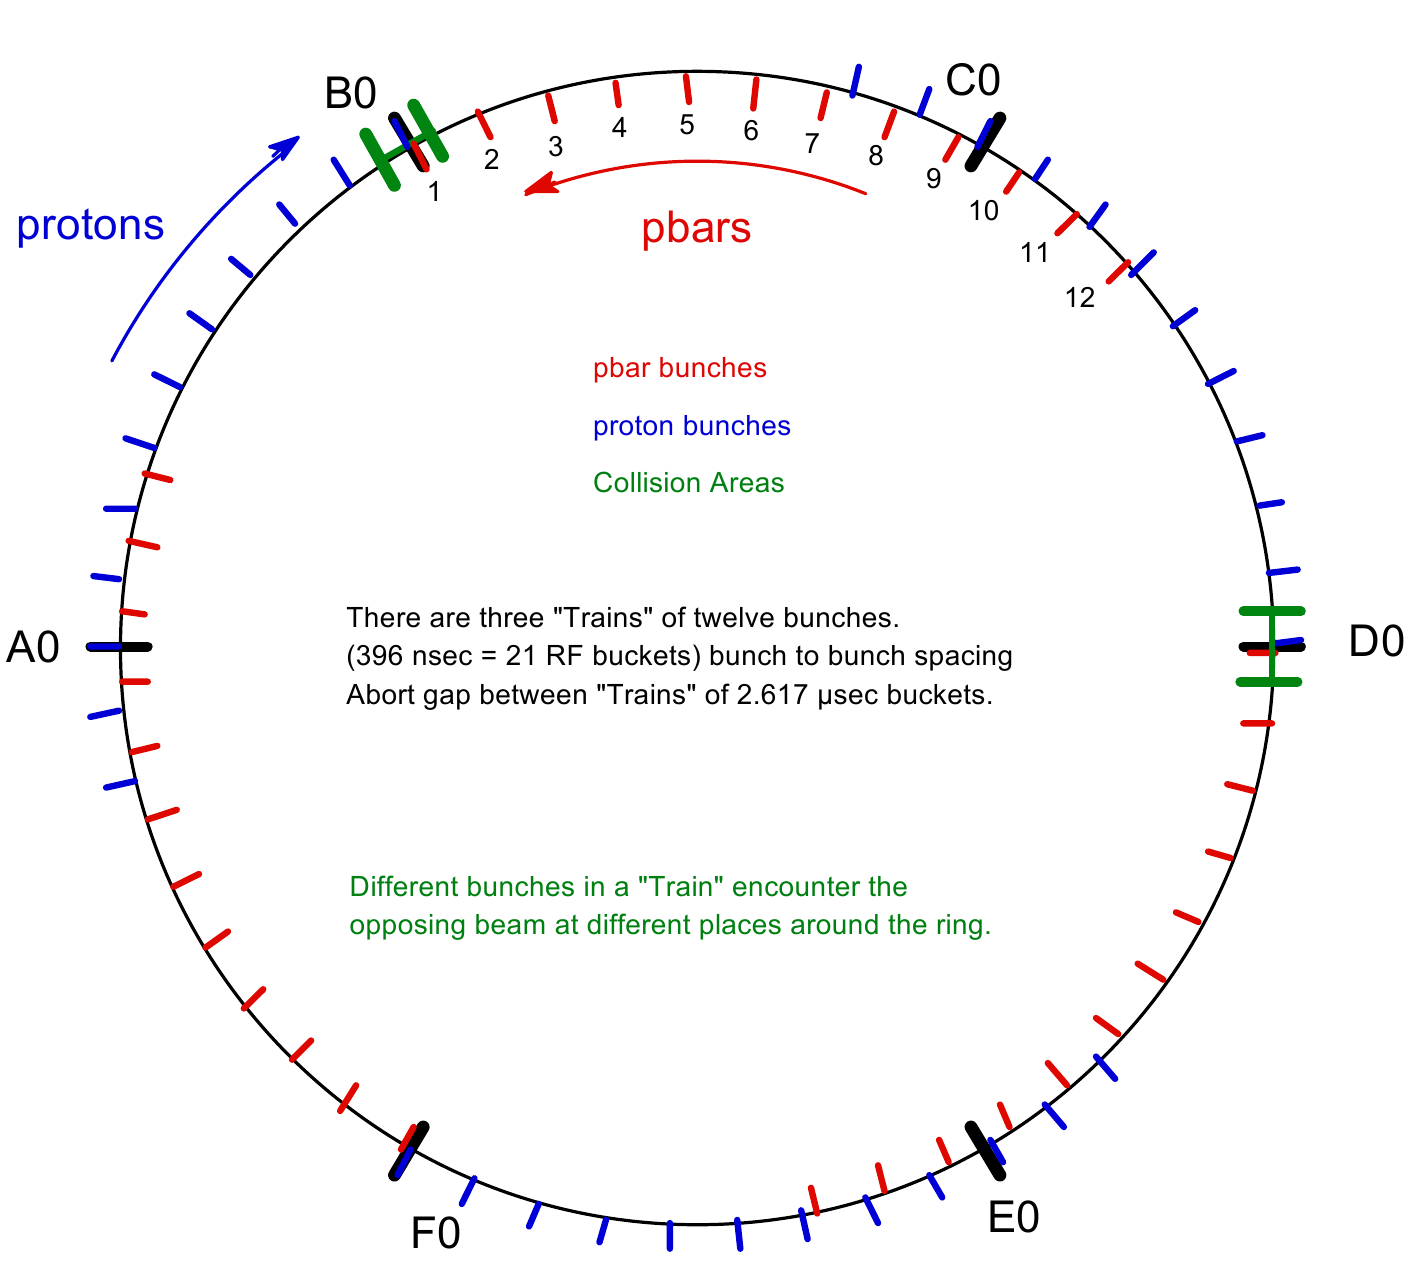
\includegraphics[scale=0.4,keepaspectratio=true]{./BunchStructure.png}
 % BunchStructure.png: 673x571 pixel, 96dpi, 17.80x15.11 cm, bb=0 0 505 428
\caption{Beam structure in 36~$\times$ 36 mode. Proton bunches go clockwise and are shown as blue marks outside the ring. Antiprotons go counterclockwise and are shown as red marks inside the ring. Detectors are located at B0 (CDF) and D0 (D\O).}
 \label{fig:BeamStructure}
\end{figure}
\vspace{-0.015\textheight}
If protons and antiprotons were orbiting in a central orbit as in Fig.~\ref{fig:BeamStructure}, the B0, D0 and F0 points would have the maximum number of collisions (12) per turn. However the present configuration is set to collide the beam at the two detectors (CDF and D\O) located at points B0 and D0. So any collisions produced at other points along the ring would be wasted. Any inefficiency is overcome by arranging the two beams into non-intersecting helical closed orbits. After the Tevatron ramps the beam energies to 980~GeV, the two beams are set in a collision helix. Several quadrupole magnets on either side of the CDF and D\O\ detectors squeeze and focus the beams to collide in the middle of the detectors.

\subsection{Instantaneous Luminosity ($\cal L$)}
Instantaneous luminosity (or simply luminosity) is a measure of the potential number of particle interactions for colliding beams. It depends on the intensity and phase space density of the interacting beams. The proton beam has about 10$^{13}$ particles and the antiproton beam has about 2$\times10^{12}$ particles. The two beams counterrotate in the accelerator ring.
%and have a Gaussian shape.
Each proton has a probability of interacting with an antiproton traveling in the opposite direction. The production rate for a specific type of interaction is defined by integrated luminosity (${\cal L}_{int}$) $\times$ cross section ($\sigma$), where the cross section is the measure of the probability for a specific type of interaction to occur in a proton-antiproton collision. Equation~\ref{eqa:LumDef1} shows the quantities used to calculate the luminosity.
\begin{equation}
{\cal L} = f \frac{N_{p}N_{\bar p}}{4\pi A}
\label{eqa:LumDef1}
\end{equation}
where $\cal L$ is the luminosity, $f$ is the frequency of bunch crossings, $N_{p}$ and $N_{\bar p}$ are the number of protons and antiprotons in each beam, and $A$ is the average size (area) of the transverse beam.

A high luminosity will yield a large interaction rate. From the above relationship, it is evident that the luminosity increases as the intensity per bunch increases and the cross sectional area of the bunch decreases. The performance of a collider is determined by integrating the luminosity over time ($\int{\cal L}~dt$). Since 2001, the Tevatron has delivered an integrated luminosity of about \cdfTotCurrLum with an ever-increasing rate (see Fig.~\ref{fig_CDFLumi}).

\section{The CDF Detector}
The Collider Detector at Fermilab (CDF) is a 5,000-ton general purpose detector with roughly 500,000 channels of information from various tracking and calorimeter components. The CDF detector is explained in detail elsewhere \cite{pap:CDFTDR, pap:CDFdetectorOverview}.

\begin{figure}[p!]
\begin{centering}
\subfigure[Integrated luminosity as function of the store number.]
{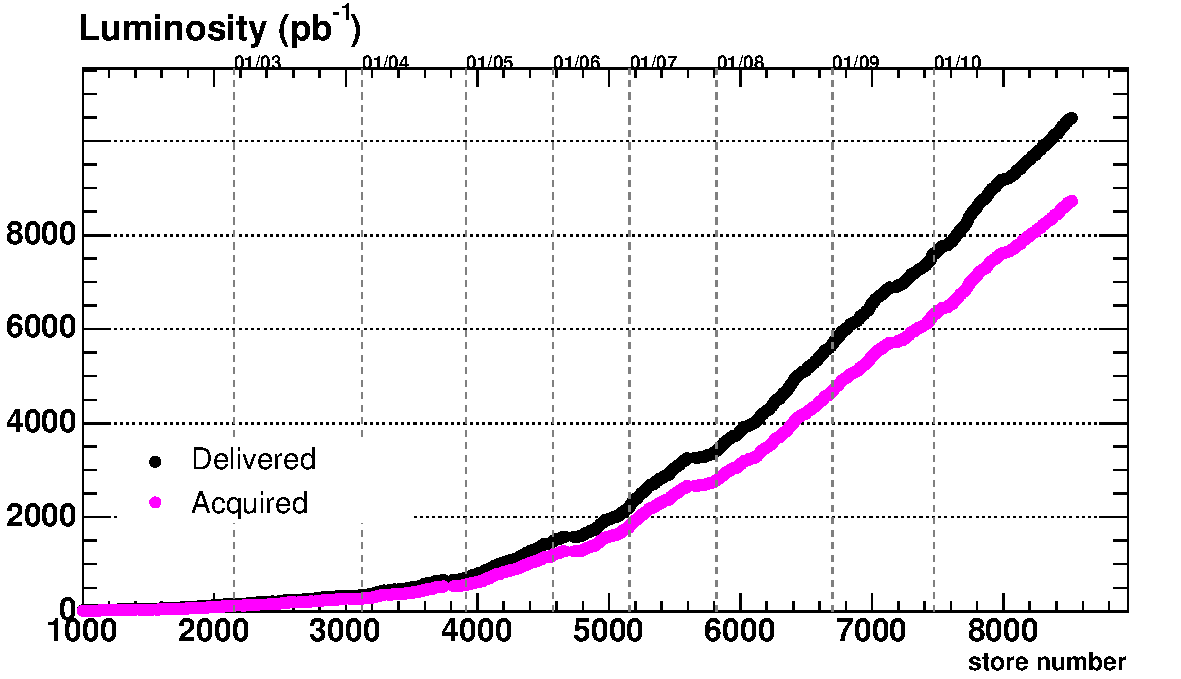
\includegraphics[scale=0.6]{CDFIntegratedLumi.pdf}
\label{subfig_lumInt}}

\subfigure[Peak instantaneous luminosity as a function of the store number.]
{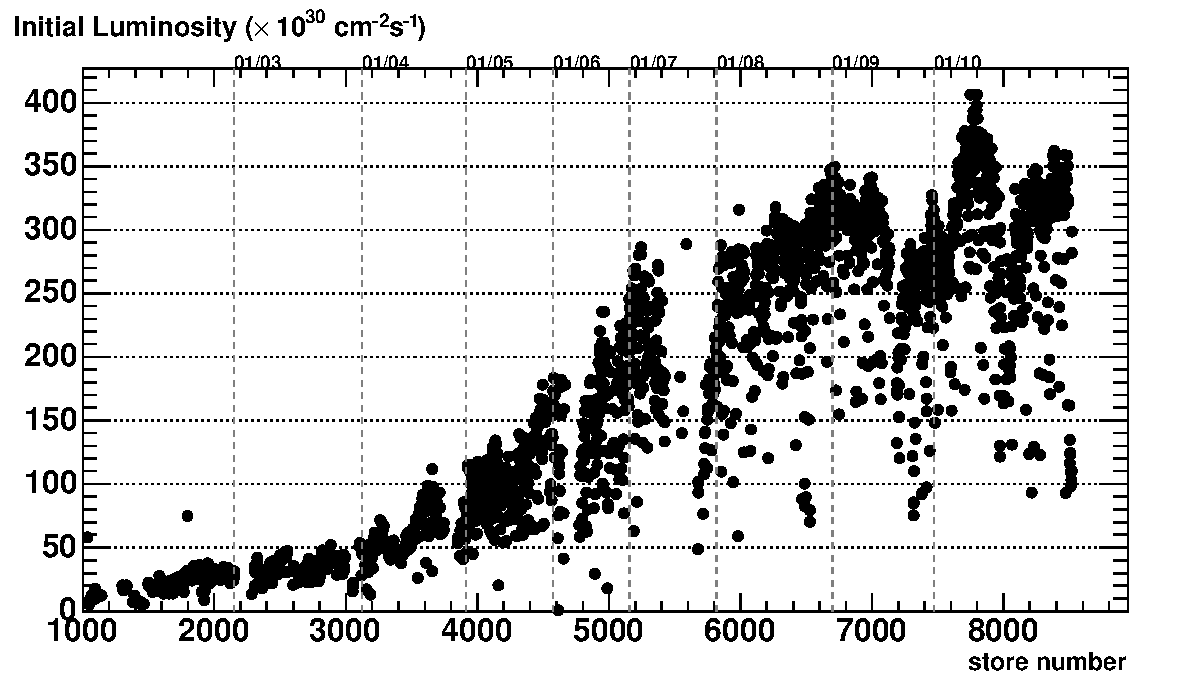
\includegraphics[scale=0.6]{CDFInitLum.pdf}
\label{subfig_lumInit}}

\caption{CDF luminosity measurements. (a) Integrated luminosity over time from 2002 to 2010 as a function of the store number, including both delivered luminosity and acquired luminosity (the amount that CDF was able to collect). This is a direct indication of the data-taking efficiency at CDF. (b) Peak instantaneous luminosity for each store over the same time period.}
\label{fig_CDFLumi}
\end{centering}
\end{figure}

At the time of writing this thesis, CDF has collected \cdfTotCurrLum~of data with a peak luminosity of around \mbox{300~$\times$ 10$^{32}$~\instLumUnits} (see Fig.~\ref{fig_CDFLumi}). A cutaway view of the CDF detector is shown in Fig.~\ref{fig_CDFdetCutAway}. The tracking system, comprised of a silicon pixel detector and open cell drift chamber, lies next to the beam pipe and is immersed in a superconducting solenoidal magnet. The amount and the direction of a deflected charged particle is used to infer its momentum and charge. Outside of the solenoid are the calorimeters, which measure the energy of particles produced in the collision. The muon detectors form the outermost layer of the CDF detector. Muons pass through the calorimeters and leave a signal in the muon chambers.

\begin{figure}[hbtm]
\begin{centering}
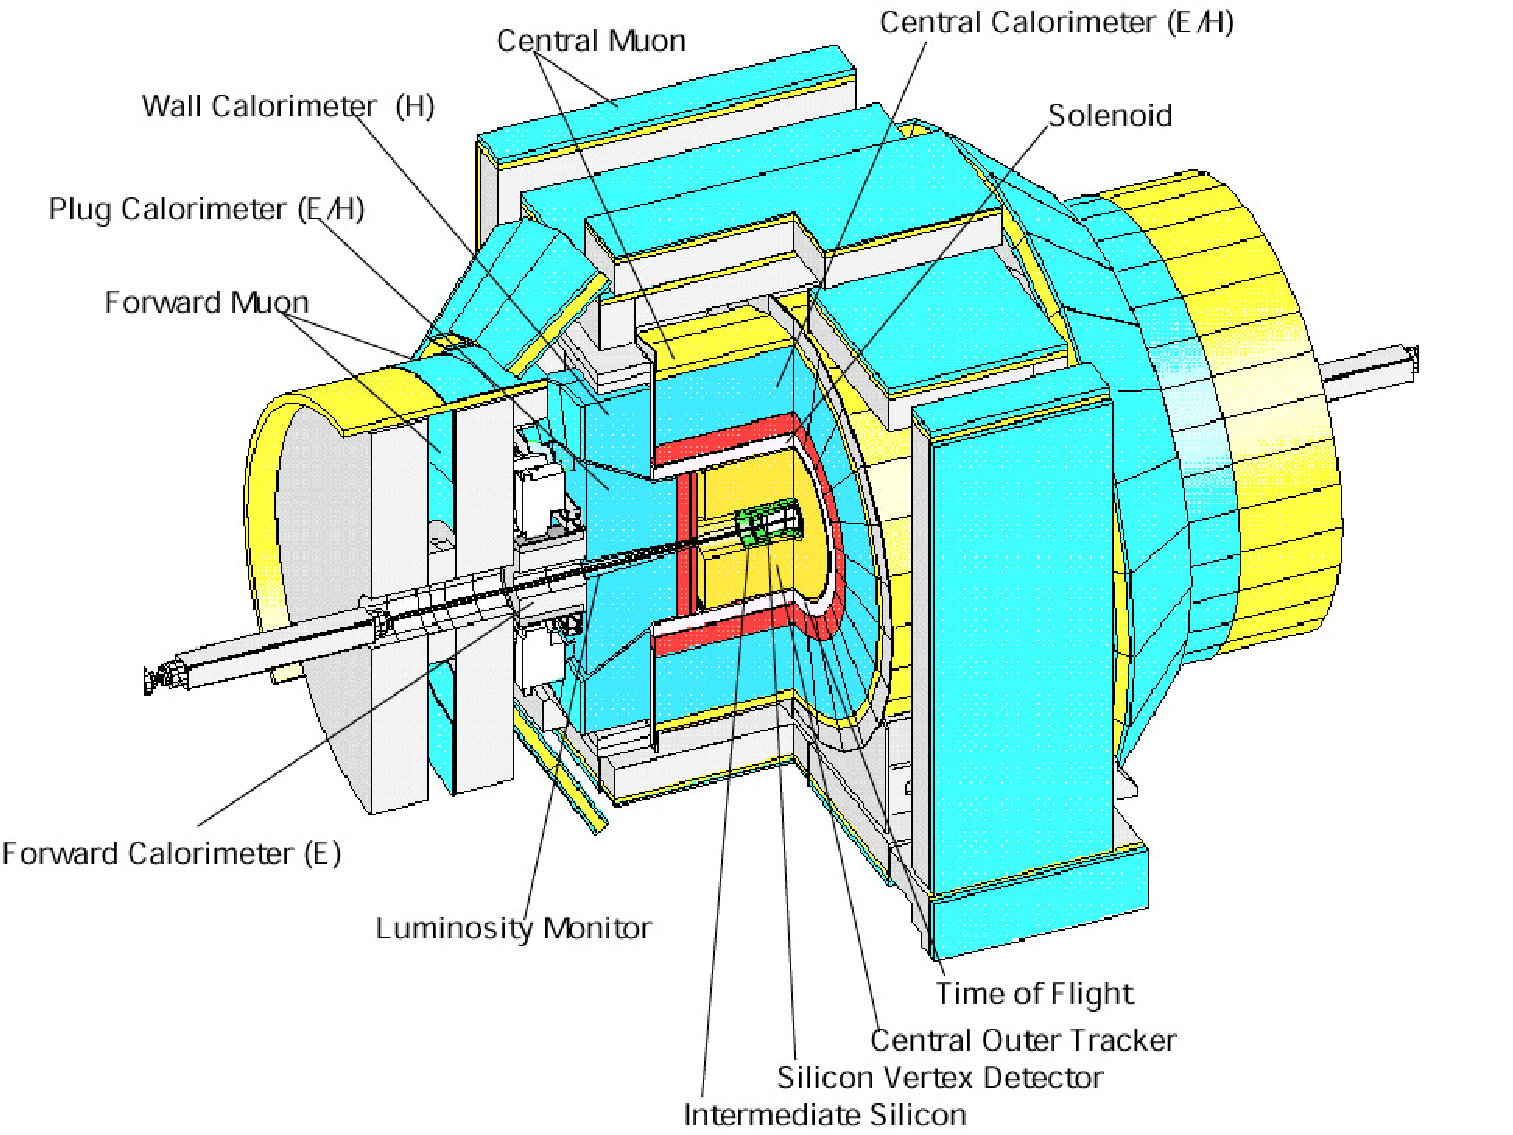
\includegraphics[scale=0.6]{CDFdetector_cutAwayView.pdf}
\caption{Cutaway view of the CDF detector.}
\label{fig_CDFdetCutAway}
\end{centering}
\end{figure}

The CDF detector is a combination of many subdetectors designed to detect certain properties of different particles and to completely reconstruct the collision event. Fig.~\ref{fig:particledecay} is a sketch of typical particle interactions in different subdetectors. The tracking chamber is the closest to the interaction point and the muon chamber is the furthest. All electrically-charged particles will leave trails in the tracking chamber. A photon, which has no electric charge, will not leave any mark in the tracking chamber but will deposit energy in the electromagnetic calorimeter. An electron is similar to a photon in the detector except that it will have an associated track. A muon, which is weakly interacting, has a longer mean lifetime than other leptons and escapes the detector leaving only a trail of hits along its path. A hadron, like the proton, will have a track and deposit the bulk of its energy in the hadron calorimeter. A neutral hadron like the neutron (\particle{n}), will show no tracks but deposit energy in the hadron calorimeter. The CDF detector exploits these simple distinctions to identify different particles and their properties.

\begin{figure}[htbm]
\begin{centering}
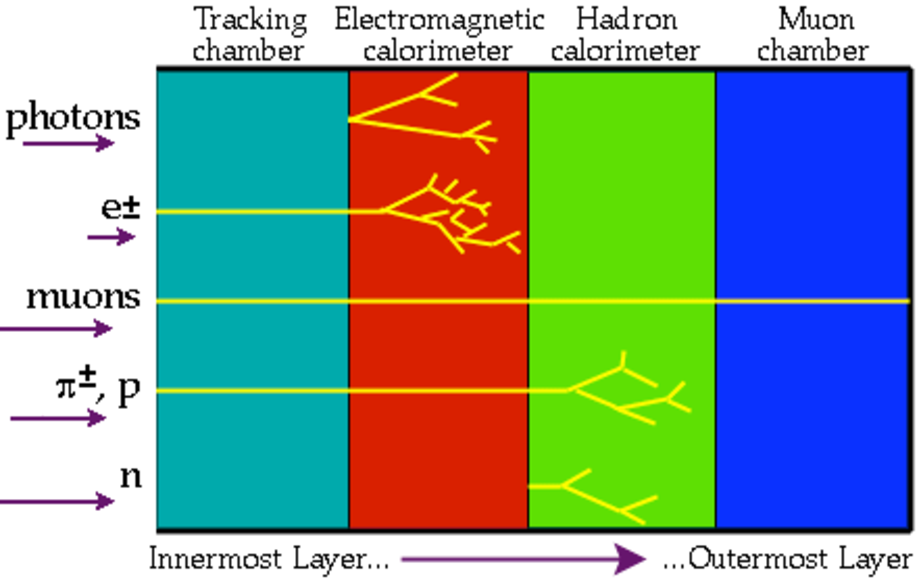
\includegraphics[scale=0.7]{decay_chart.pdf}
\caption{Diagram depicting particle interactions with different detectors. These differences help
to identify and distinguish particles generated in a hard scattering process.}
\label{fig:particledecay}
\end{centering}
\end{figure}

\subsection{Coordinate System}
The coordinate system used to describe the location of different components in the CDF detector is illustrated in Fig.~\ref{fig:cdfCDTsystem} and described below.

\begin{figure}[htbm]
 \centering
 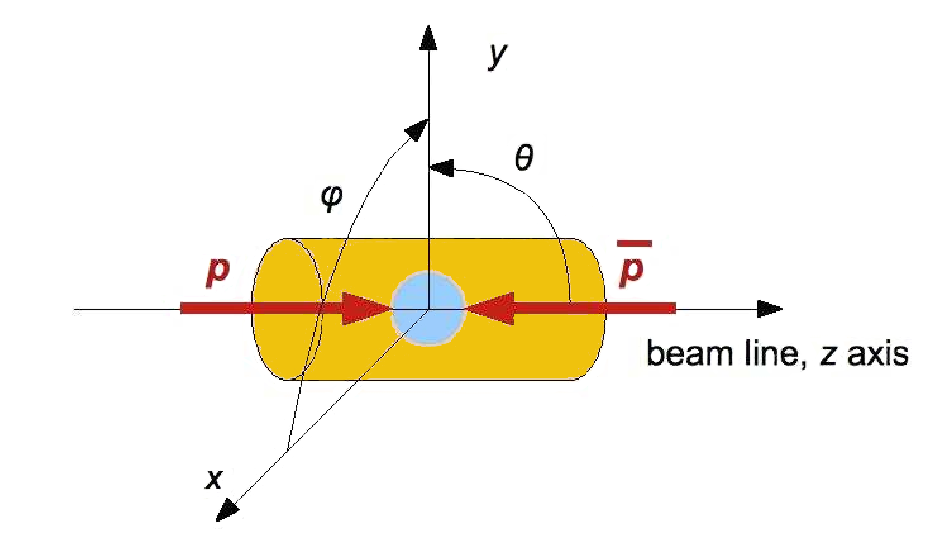
\includegraphics[scale=.5]{./cdfCoordinateSystem.png}
 % cdfCoordinateSystem.png: 937x550 pixel, 96dpi, 24.79x14.55 cm, bb=0 0 703 412
 \caption{CDF coordinate system.}
 \label{fig:cdfCDTsystem}
\end{figure}

\vspace{-0.015\textheight}
\begin{singlespace}
\begin{itemize}{}{}
\item{$z$ = Distance along the beamline. Protons travel in the $+z$ direction (east) and antiprotons travel in the $-z$ direction (west). $z=0$ is the interaction point (IP).}
\item{$r$ = Radial distance from the beamline.}
\item{$\theta$ = Polar angle from the beamline. \mbox{$\theta$ = 0\degree} is the $+z$ direction, \mbox{$\theta$ = 90\degree} is straight up, and \mbox{$\theta$ = 180\degree} is the $-z$ direction. Typically $\eta$, as described below, is used instead of $\theta$.}
\item{$\eta$ = Pseudorapidity, which is defined as $-\ln(\tan(\theta/2))$, so particles perpendicular to the beamline have $\eta = 0$. The beamline itself has an $\eta$ of $+\infty$ in the $+z$ direction and $-\infty$ in the $-z$ direction. \mbox{$\theta$ = $\pm$45\degree} corresponds to \mbox{$\eta=\pm$0.88}.}
\item{$\phi$ = Azimuthal angle around the beamline. North is \mbox{$\phi$ = 0}, up is \mbox{$\phi$ = 90\degree}, south is \mbox{$\phi$ = 180\degree}, and down is \mbox{$\phi$ = 270\degree}.}
\end{itemize}
\end{singlespace}

The CDF detector is left-right and cylindrically symmetric with few exceptions. Many components in the CDF detector are segmented into \mbox{15-degree} wedges in $\phi$. These wedges are numbered with 0 at \mbox{$\phi$=0}, proceeding in the \mbox{+$\phi$} direction. Usually, a wedge refers to a given $\phi$ segment on a given east/west side of the detector; for example, wedge 0E refers to the wedge from \mbox{0--15} degrees $\phi$ on the east side of the detector, and wedge 0W refers to the wedge from \mbox{0--15} degrees $\phi$ on the west side of the detector. The CDF detector is further classified into three regions of pseudorapidity, \newterm{central} (\etalessthan{1.1}), \newterm{plug} (\etaabsregion{1.1}{3.6}), and \newterm{forward} ($|\eta|>3.6$). Figure \ref{fig:EtaRegionsTowerGeometry} shows a schematic view of a quarter of the CDF detector. It shows the projective tower geometry and the relative location of the subdetectors.

\begin{figure}[htb!]
 \centering
 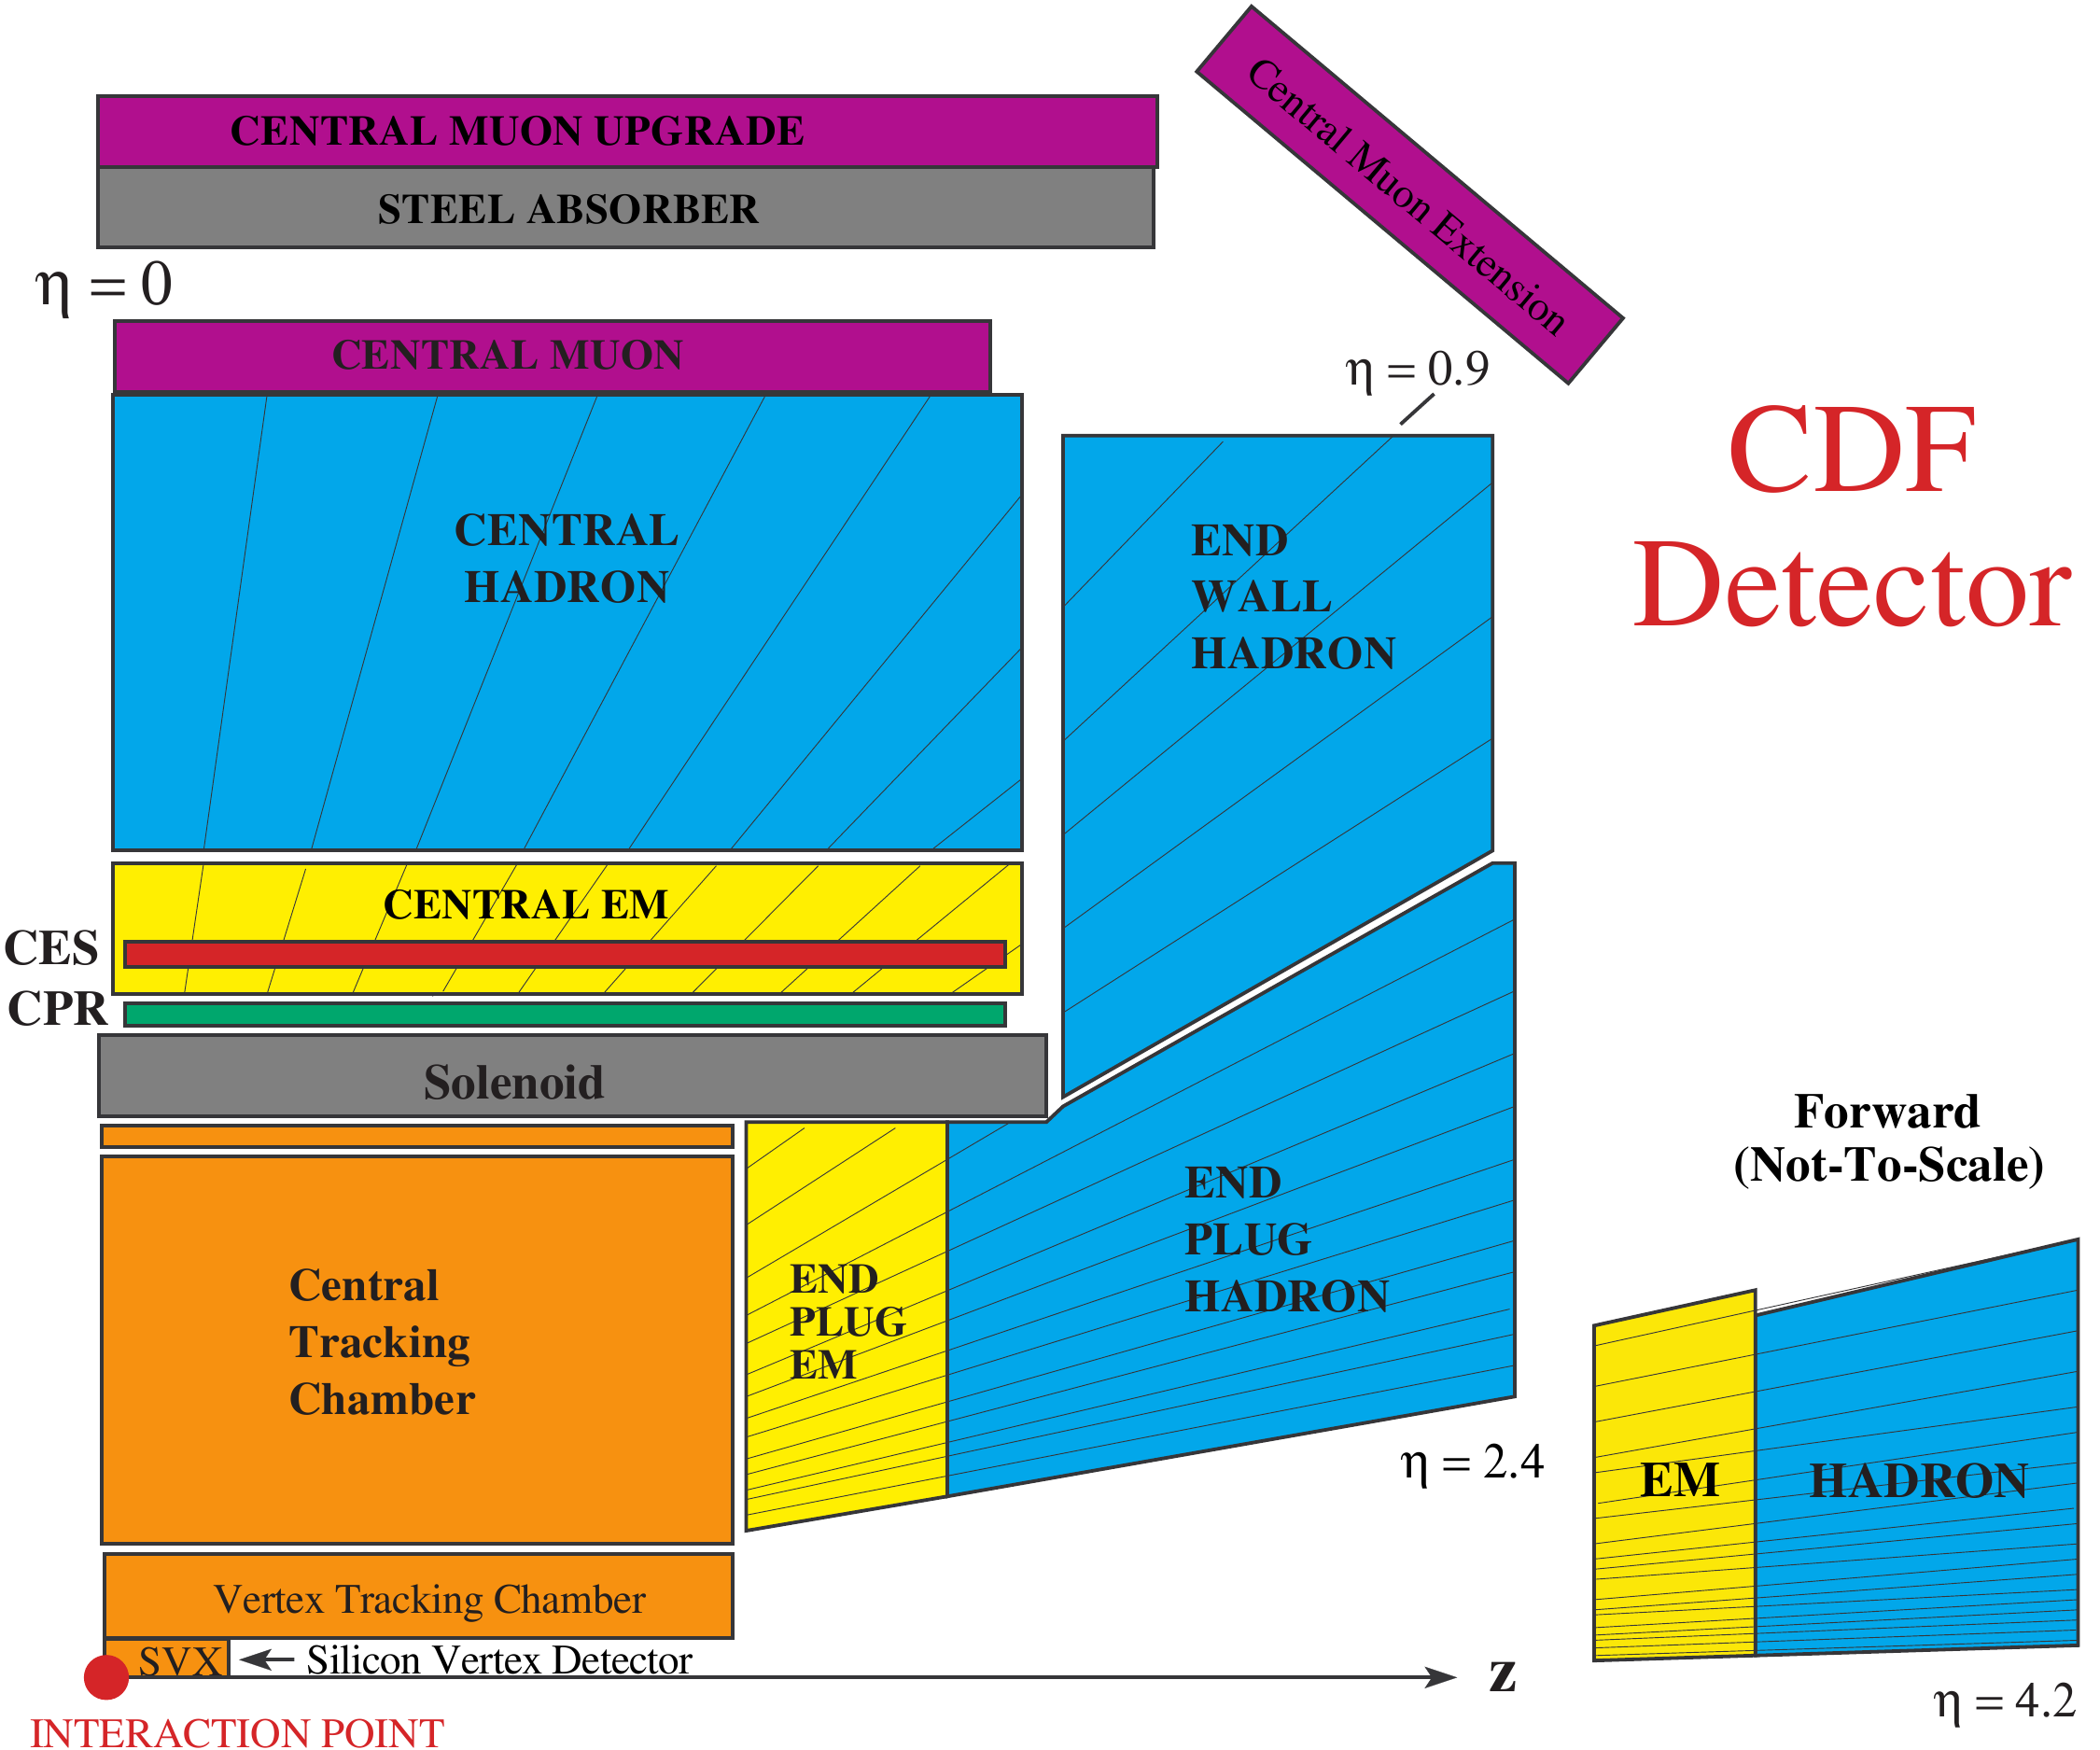
\includegraphics[scale=0.24]{./CDF_ColorQuarter_TowerGeometry.png}
 % CDF_ColorQuarter_TowerGeometry.png: 2250x1875 pixel, 96dpi, 59.52x49.60 cm, bb=0 0 1687 1406
 \caption{A quarter view of the CDF detector indicating the location of different subdetectors with respect to the nominal collision (interaction) point. $\eta$-regions and the projective tower geometry are indicated by lines extending from the interaction point.}
 \label{fig:EtaRegionsTowerGeometry}
\end{figure}


\subsection{Luminosity Counter}
The CDF detector is equipped with high-yield gaseous Cherenkov counters for precise measurement of the luminosity. Located close to the beamline (\etaabsregion{3.7}{4.7}), it measures the Cherenkov radiation (light) from the inelastic collisions (see Fig.~\ref{fig_CLC_Assembly}). The light measured is proportional to the number of inelastic collisions \cite{pap:CLCperformance}. The luminosity can be calculated using
\begin{equation}
%\lum \mathrm{= \frac{\mu \times f_{BC}} {\sigma _{in}} }
{\cal L} = \frac{\mu \cdot f_\mathrm{BC}}{\sigma_{\mathrm{in}}},
\label{eqa:LumDef2}
\end{equation}
where $\cal L$ is the instantaneous luminosity, $f_\mathrm{BC}$ is the rate of bunch crossings (1.7~MHz), $\mu$ is the average number of \ppbar interactions per bunch crossing, and $\sigma_\mathrm{in}$ is the inelastic cross section (=~60~mb).


\begin{figure}[htb!]
\begin{centering}
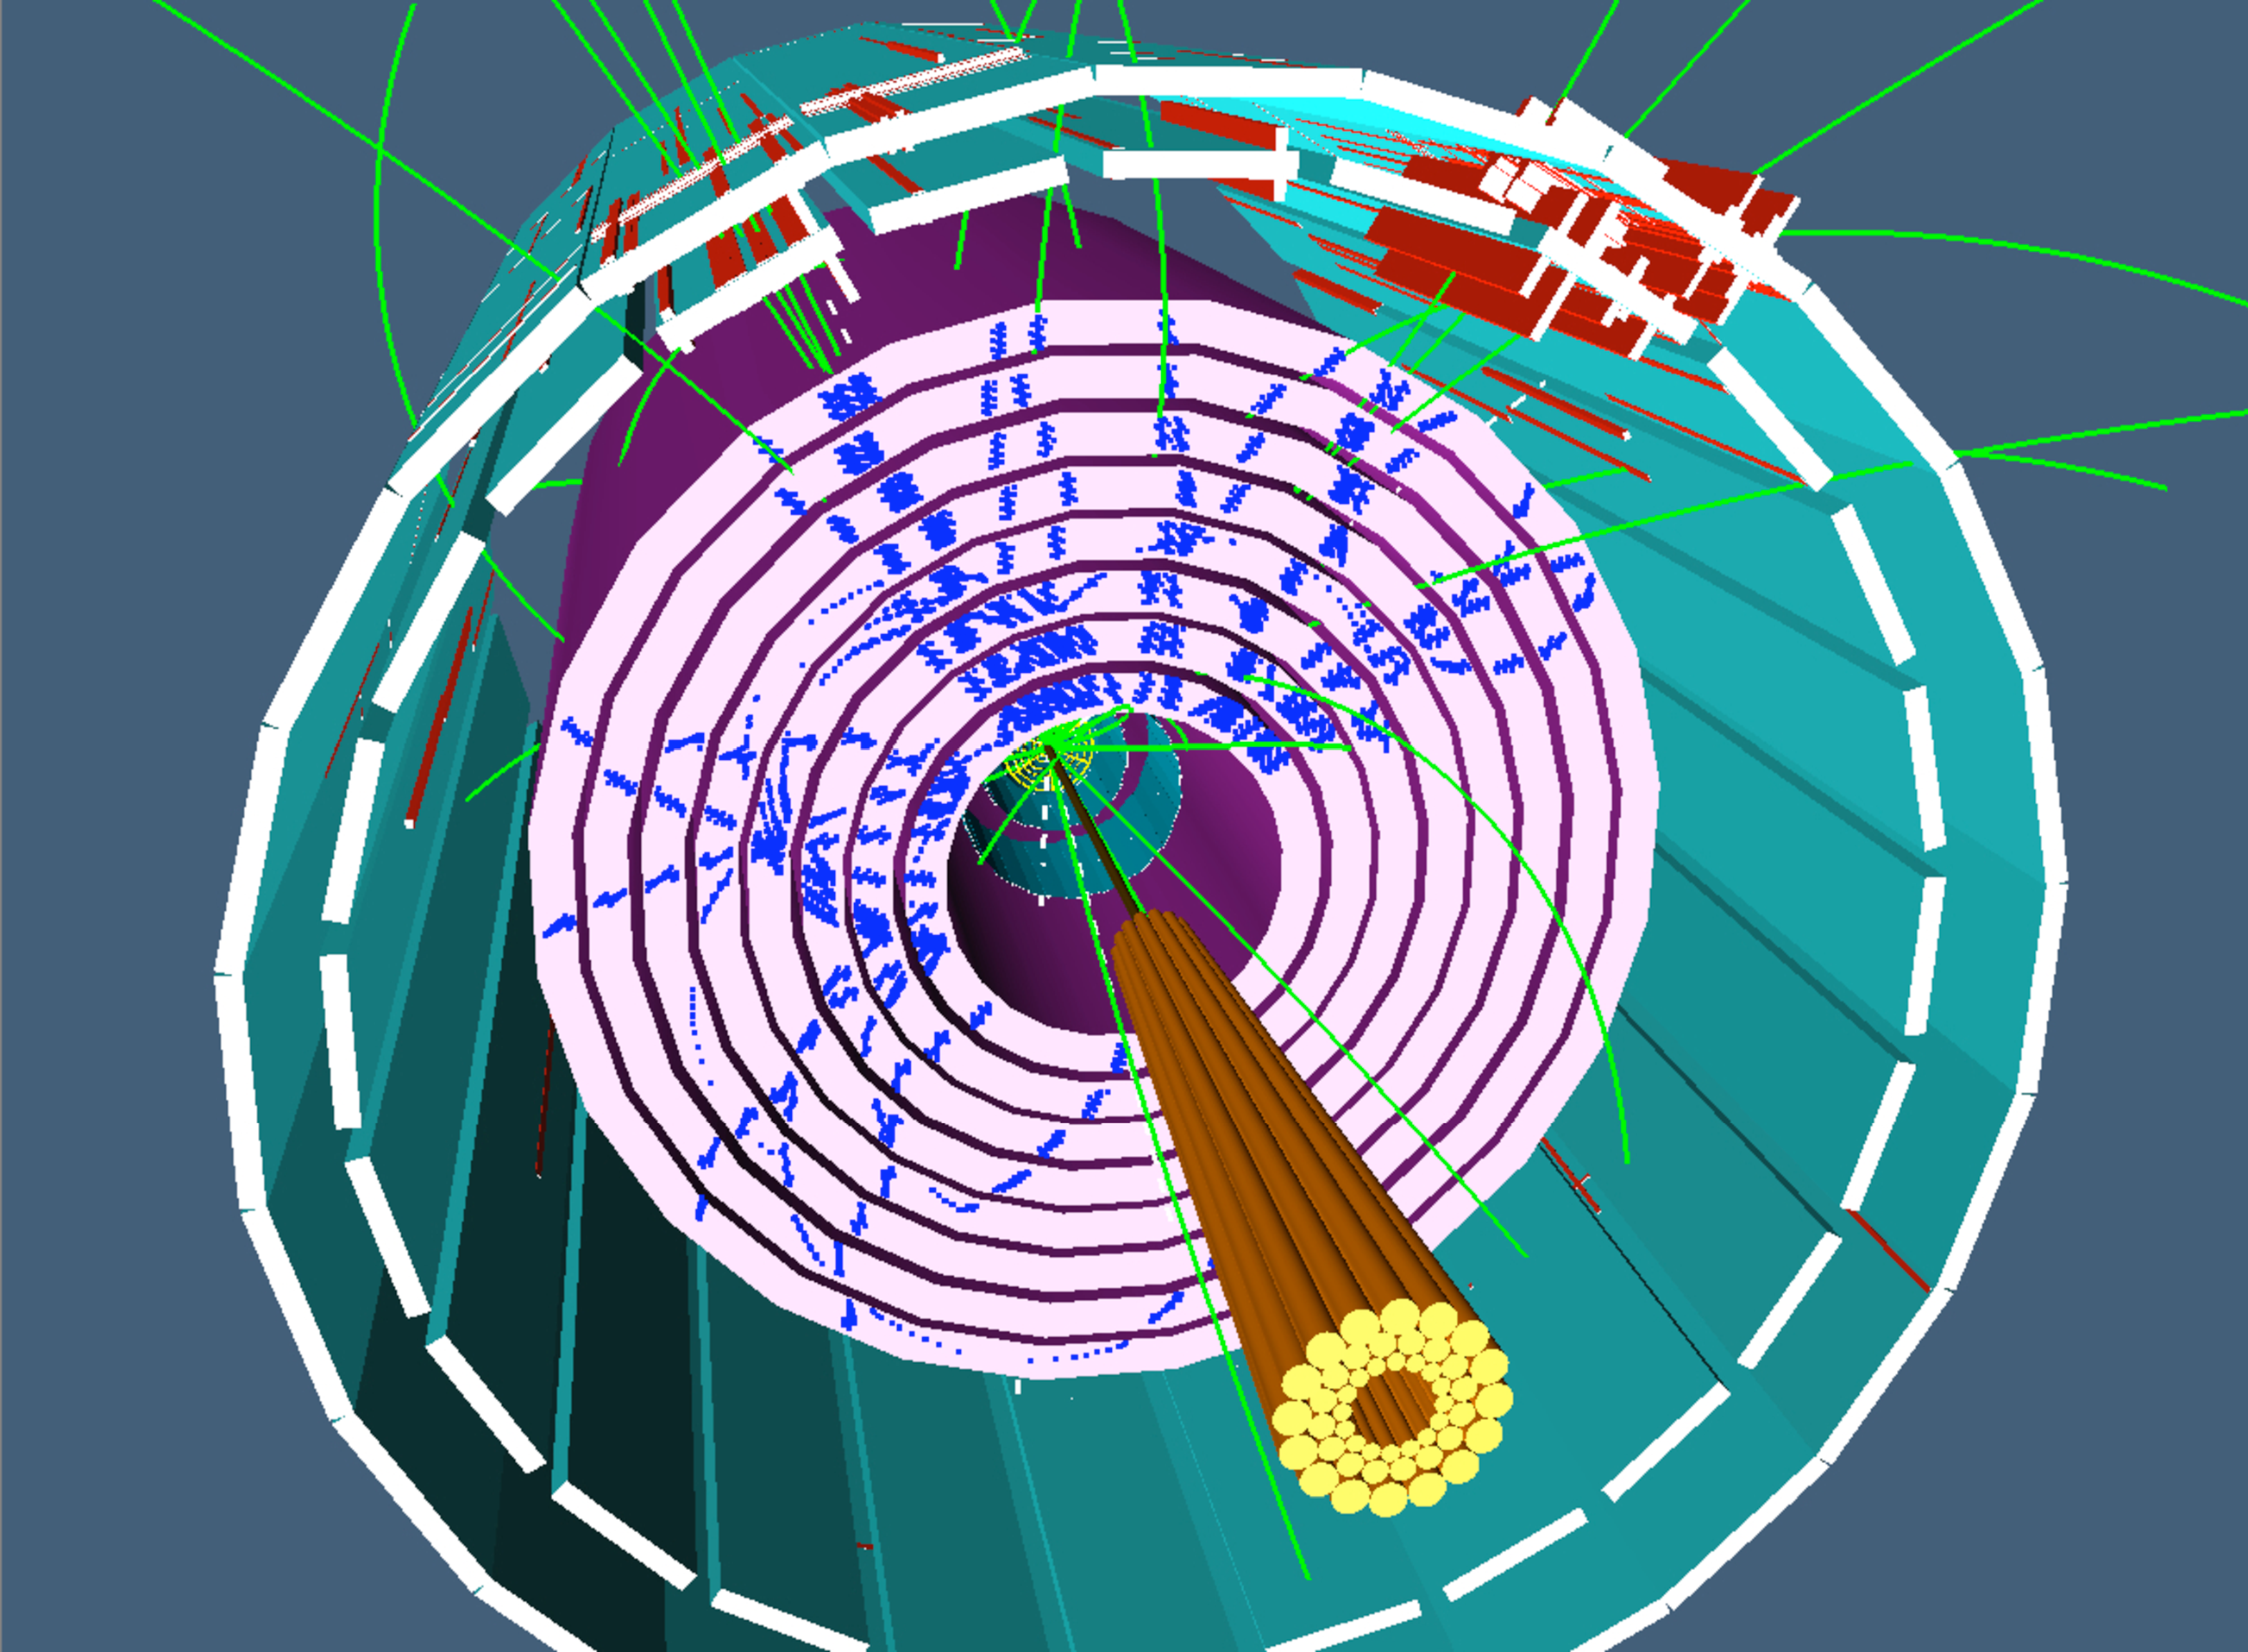
\includegraphics[scale=0.3]{CLC_withTracks.pdf}
\caption{Graphic depicting the CLC detector (in brown).}
\label{fig_CLC_Assembly}
\end{centering}
\end{figure}


\subsection{Solenoid}
The CDF tracking volume is immersed in a 1.4~T magnetic field generated by a 5~m long Nb-Ti superconducting solenoid. The magnetic field is aligned along the direction of the beam pipe so it does not deflect the protons or antiprotons circling in the Tevatron. Secondary particles from the collisions traveling perpendicular to the beam pipe are deflected by the magnetic field according to the Lorentz force law, $\vec{F}=q\vec{v}\times \vec{B}$. This allows the tracking detectors to measure the momenta of particles and the sign of their charge.

\subsection{Tracking System}\label{sec:TrackingSystem}
A well equipped high-precision charged-particle tracking system is used at CDF. It is comprised of an open cell drift chamber, the Central Outer Tracker (COT), and a set of silicon layers laid inside the COT close to the beam pipe (see Fig.~\ref{fig:TrackingCoverage}). A micro-vertex detector close to the beam pipe measures the impact parameter resolution. A set of intermediate silicon strips enhances the vertex and track reconstruction. The silicon strips, when combined with the COT tracks, increase the \pt resolution and are used for $b$-tagging in the forward region. When used alone, the silicon detector provides tracking over the full region of \mbox{$|\eta|\leq2.0$}. This state-of-the-art tracking system is at the heart of many analyses performed at CDF.

\begin{figure}[htb!]
\begin{centering}
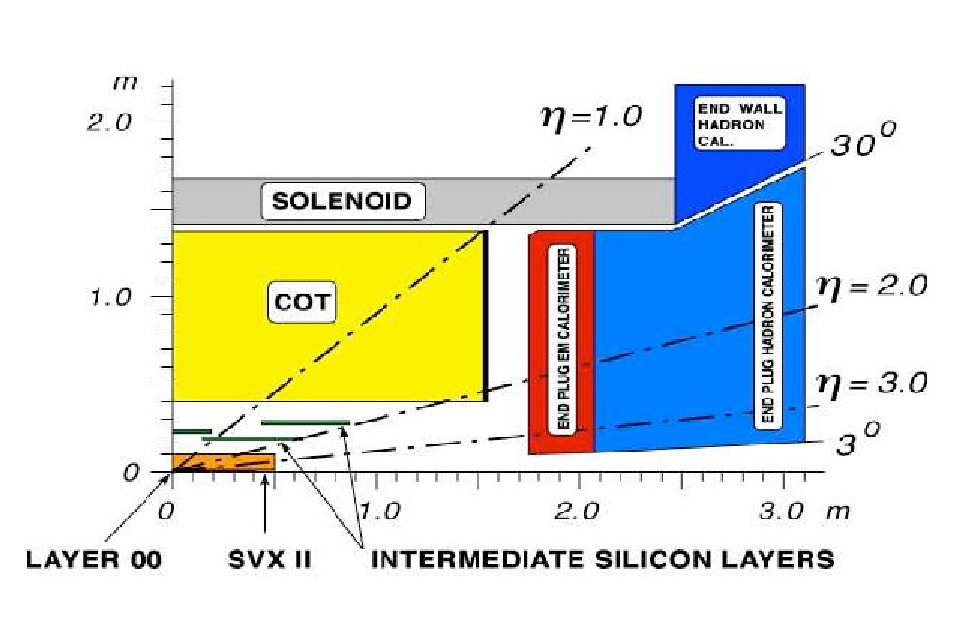
\includegraphics[scale=0.95]{CDF_TrackingCoverage.pdf}
\caption{Tracking coverage of the CDF detector. The figure only shows 1/4 of the detector. The nominal collision point is at coordinate (0,0).
}
\label{fig:TrackingCoverage}
\end{centering}
\end{figure}

\subsubsection{Silicon Tracking}\label{sec:SiliconTracking}
Nine layers of silicon micro strips measure the $x$, $y$ and $z$ positions of the charged particles produced in a collision \cite{pap:SiliconDetector}. They lie next to the beam pipe and comprise 3 detector subsystems. The first silicon layer, Layer 00 (L00), is mounted on the beampipe. The next five silicon layers make up the Silicon Vertex Detector (SVX-II) (Fig.~\ref{fig_SvxEndView}). And the last three make up the Intermediate Silicon Layers (ISL) which cover the region \etalessthan{2}. The L00 detector enhances the vertex and tracking capabilities and has a 11~micron hit resolution. The main purpose of the SVX-II is high-precision tracking and secondary vertex detection. The SVX-II has a position resolution of $\sim$9 microns for 2-strip clusters. The SVX-II and ISL together provide stand-alone silicon tracking and are vital for $b$-tagging. The single hit resolution is \mbox{$\leq16~\mu m$} on the axial side and $\leq$~23~$\mu$m on the stereo side. The silicon system's impact parameter resolution is approximately 40~$\mu$m.

\begin{figure}[htb!]
\begin{centering}
\raisebox{0.25\height}{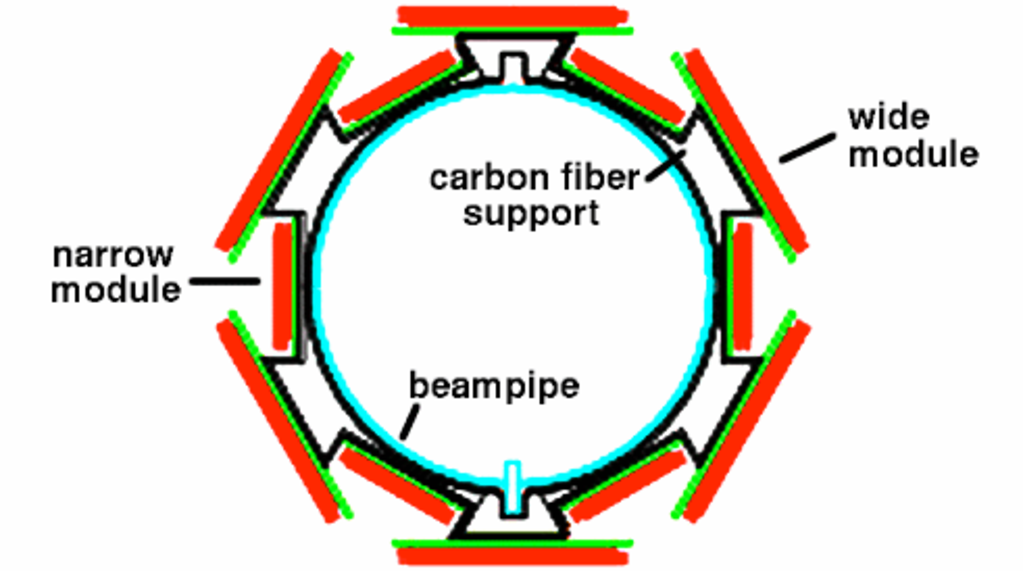
\includegraphics[scale=0.4]{L00EndView.pdf}}
\hspace*{.2in}
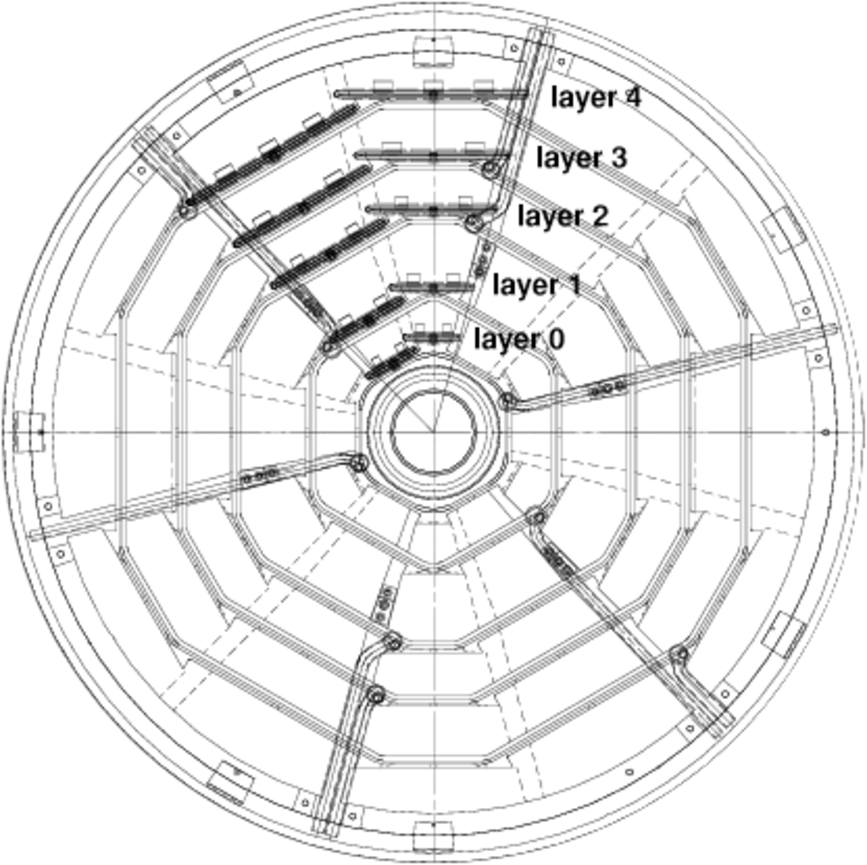
\includegraphics[scale=0.4]{SvxBulkHeadEndView.pdf}
\caption{End view of the Layer 00 silicon detector (left), and end view of the SVX-II silicon vertex detector (right).}
\label{fig_SvxEndView}
\end{centering}
\end{figure}

\subsubsection{Central Outer Tracker (COT)}\label{sec:COT}
The COT \cite{pap:COT} is an open cell drift chamber providing complete charge particle tracking coverage over the region \mbox{$|\eta|\leq1.0$} and partial coverage up to \etalessthan{2}. It has a inner radius of \mbox{44 cm}, a outer radius of \mbox{132 cm}, and spans about 3~m in length along the beamline ($z$). The complete chamber is roughly 1.3\% of a radiation length at normal incidence. A total of 2520 cells called \newterm{supercells} are arranged to form 8 layers called \newterm{superlayers} (SL) to reconstruct tracks with high precision and purity. Cells across layers are designed to have approximately the same maximum drift distance, and the number of cells increases with radius as seen in Fig.~\ref{fig:COT_endview}. Cells are filled with fast-response ionizing gas which limits drift times to less than 100~ns. A drift cell has a line of 12 sense wires and 12 shaper wires placed alternatively in the middle of the cell (Fig.~\ref{fig:COT_cells}). The superlayers are arranged in alternating \newterm{axial} and \newterm{stereo} layers. Axial super layers have the wires in the cells running parallel to the $z$ axis. Wires in the stereo layers are shifted by a 3\degree angle with respect to the $z$ axis. This provides an apparent shift in the charge particle track to give a 3-dimensional view of the tracks. The combination of axial and stereo layer information provides the $z$ and $r-\phi$ positions.

\begin{figure}[htb!]
 \centering
 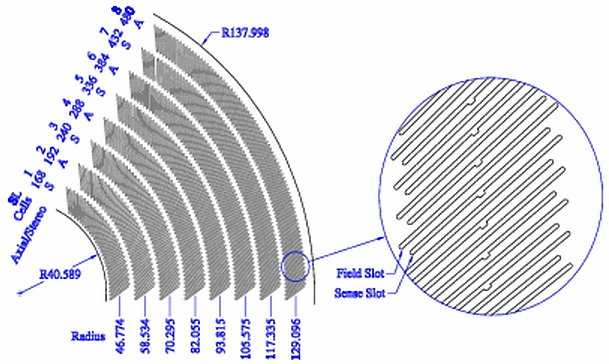
\includegraphics[keepaspectratio=true,scale=0.6]{./cot_end.png}
 % cot_end.png: 609x364 pixel, 72dpi, 21.48x12.84 cm, bb=0 0 609 364
 \caption{A section of 1/6 of the COT end plate. The information given for each superlayer is the total number of supercells, the wire orientation (axial or stereo), and the average radius in centimeters. The enlargement shows the sense and field slot geometry in detail.}
 \label{fig:COT_endview}
\end{figure}

\begin{figure}[htb!]
 \centering
 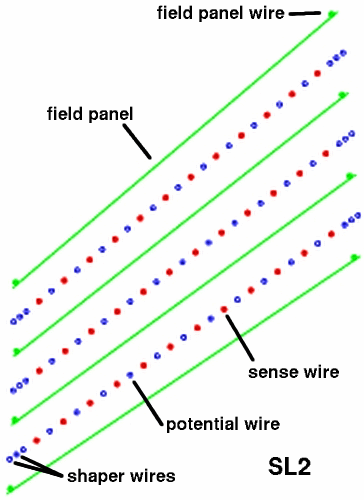
\includegraphics[keepaspectratio=true,scale=0.8]{./cot_cells.png}
 % cot_cells.png: 364x500 pixel, 72dpi, 12.84x17.64 cm, bb=0 0 364 500
 \caption{Three COT cells in superlayer 2 looking down along the beamline, $z$. Note that some details are not to drawn to correct scale.}
 \label{fig:COT_cells}
\end{figure}

% Table not complete ##############################
% SEE Nucl. Inst. Meth A 42586
% \begin{table}
% \centering
% \begin{tabular}{cc}
% \hline
% {\bf } & {\bf Momentum Resolution $\sigma(p_{T})/p_{T})$}\\
% \hline
% COT alone & 0.15\% |\\
% \end{tabular}
% \caption{Momentum resolution when COT and Silicon tracking systems are combined.}
% \label{tab:COTMomentumResolution}
% \end{table}

\subsection{Preshower Detector}\label{sec:CPR}
The preshower detector is used to sample the particles before they reach the calorimeter. As there is lot of material (the COT, the magnet) in between the calorimeter and the interaction point, particles such as photons can convert in material (for example, $\gamma\to e^{+}+e^{-}$). The preshower detector acts as a redundant measurement for particle identification. In Run II, the gas-filled preshower detector was replaced with a fast-response low-noise scintillator tile detector (see Fig.~\ref{fig:CPRtile}). Unlike the old detector, the new detector has no dead regions. A continuous array of 3~$\times$ 18 tiles (12.5~$\times$~12.5~cm$^2$ each) spans the face of one calorimeter wedge. It samples the early particle shower in front of the central calorimeter (see Fig.~\ref{fig_cprlocation}). The preshower detector can be used to efficiently identify single photons from light meson decays (\textit{e.g.} $\pi^{0}\rightarrow\gamma\gamma$) to improve photon measurements \cite{pap:CPRdetector}. Above 35~GeV, photons from light meson decays cannot be resolved using only the shower maximum detector (see Section~\ref{sec:CES}) because the angular separation of the two photons is too small. This new scintillator detector is designed to measure single particles and requires more then 5 photo electrons per minimum ionization particle (MIP).

\begin{figure}[htb!]
 \centering
 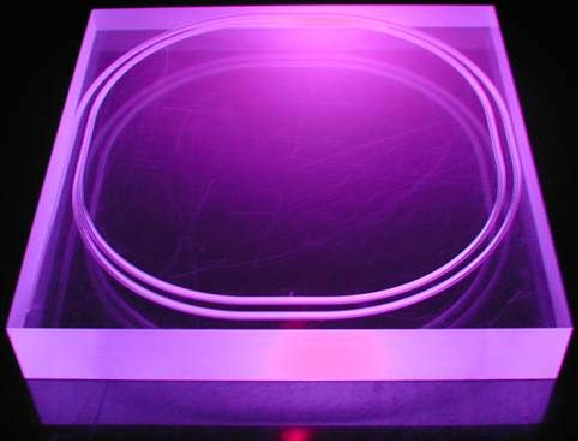
\includegraphics[scale=.5]{./CPRtile.png}
 % CPRtile.png: 578x441 pixel, 96dpi, 15.29x11.67 cm, bb=0 0 433 331
 \caption{A scintillator tile used in the new preshower detector. The tile is carved with a two-loop spiral groove in which a wavelength-shifting (WLS) fiber is embedded. The fiber carries out the light produced by the tile.}
 \label{fig:CPRtile}
\end{figure}


\begin{figure}[htb!]
\begin{centering}
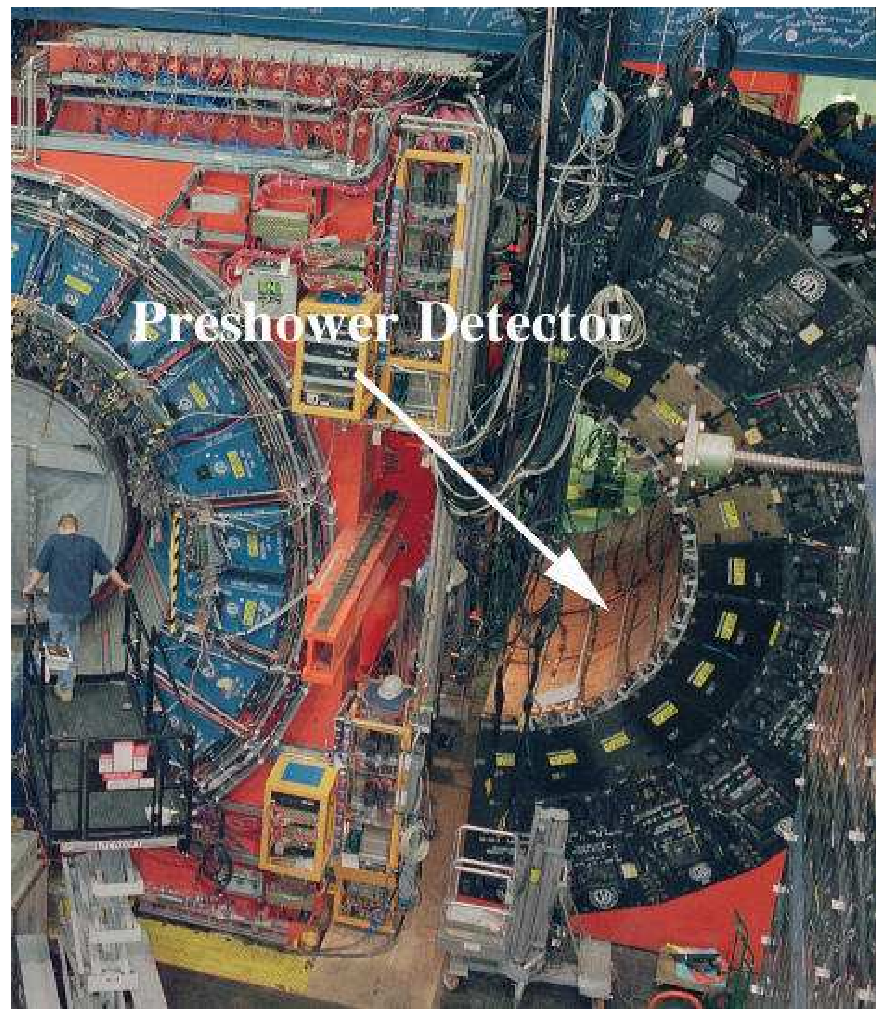
\includegraphics[scale=0.35]{CPR_Location2.png}
\caption{Photo of a section of the CDF detector before the new preshower detector installation. One of the calorimeter arches is open for maintenance, and twelve calorimeter wedges are visible. On the inner surface of each of the calorimeter wedge lies an array of scintillator tiles for the preshower detector.}
\label{fig_cprlocation}
\end{centering}
\end{figure}

\begin{figure}[htb!]
 \centering
 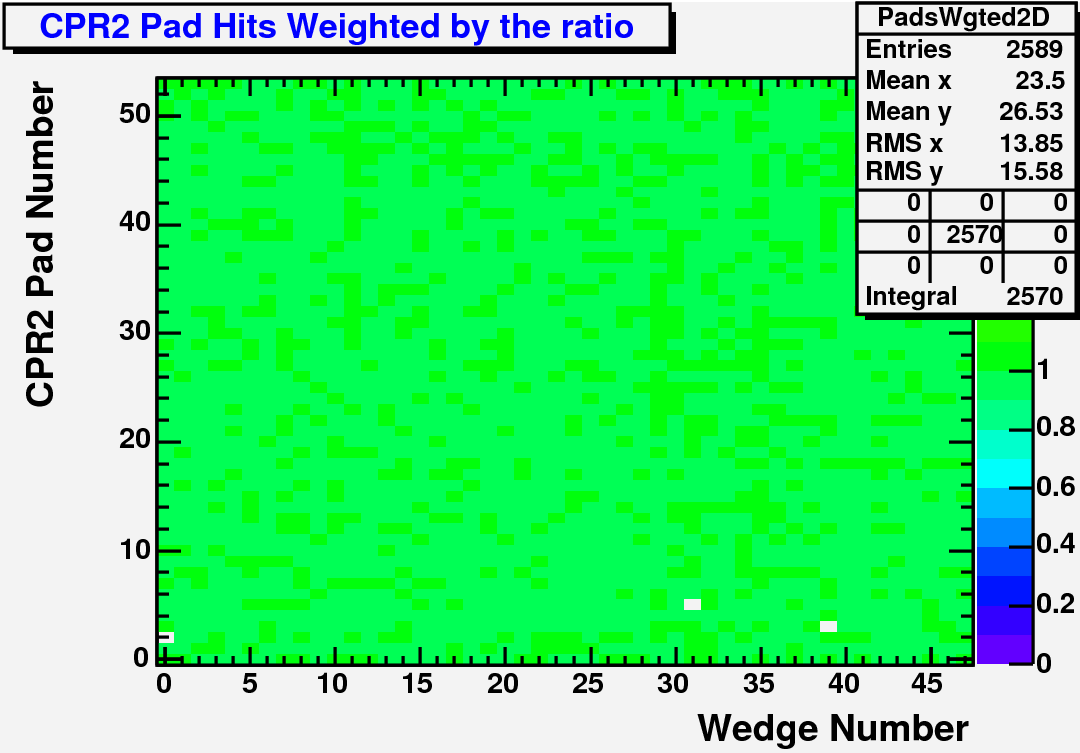
\includegraphics[scale=0.35,keepaspectratio=true]{./CPRcalibration1.png}
 % CPRcalibration1.png: 1080x753 pixel, 96dpi, 28.57x19.92 cm, bb=0 0 810 565
 \caption{A histogram used in the calibration process to check the energy gain of CPR tiles. The \newterm{dead} channels show up in white. Each tile's gain is compared to the global response, and tiles with low gain will show up in warm colors.}
 \label{fig:CPRcalibration}
\end{figure}

The author was part of the offline calibration group that provided calibration information on the CPR detector. Due to radiation damage and aging of the scintillator tiles, their photoproduction diminishes over time and the response to MIPs needs to reevaluated. For this, every CPR channel's gain is adjusted for each run period. A sample calibration plot of the CPR detector is shown in Fig.~\ref{fig:CPRcalibration}. Furthermore, the CPR detector status (whether it was on and functioning properly during data-taking) was determined by measuring the occupancy and reported to the Data Quality Monitoring (DQM) group. This information is used to determine whether certain data is useful for physics analysis (see Section~\ref{sec:GoodRun}).

\subsection{Calorimeter System}\label{sec:Calorimeter}
The calorimeter system is located outside of the solenoid and it is a tower-segmented scintillator sampling calorimeter. The calorimeter has a projective tower geometry (see Fig.~\ref{fig:EtaRegionsTowerGeometry}) where each tower is 15\degree in azimuth by about 0.11 in pseudorapidity. Each wedge consists of a lead-scintillator electromagnetic calorimeter section backed by a steel-scintillator hadron calorimeter \cite{pap:CDFTDR}. The central calorimeter system extends to \etaregion{-1.1}{1.1} and the plug calorimeter to \etaabsregion{1.1}{3.6}. Calorimeter information is read out via mounted fast PMTs. The central calorimeters are read out with two photo-multipliers, located on either side of tower, whereas the plug calorimeter towers are equipped with one PMT. It will be explained later that the two PMT readouts are vital in the central calorimeter for identifying fake photons that arise due to random energy fluctuations in the PMTs.

The calorimeter is designed to sample and measure particle energies. It can also provide a very coarse direction measurement of the particles and aid in particle identification. When a particle enters the calorimeter, it interacts with calorimeter material, losing its energy by producing a cascade of electrons and photons which is termed a \newterm{shower}. A simulation of an electron-induced cascade is shown in Fig.~\ref{fig:ElecCascadeInIron}. The progress of the shower is measured by scintillator material embedded in between the absorbers. The shower shape and size is different for different particles, and the calorimeter response will also vary for different particles.

\begin{figure}[hbtm]
 \centering
 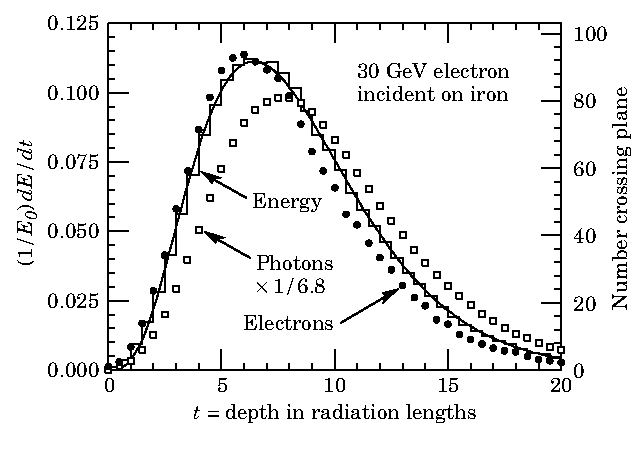
\includegraphics[scale=1.4,keepaspectratio=true]{./ElecCascadeInIron.pdf}
 % ElecCascadeInIron.pdf: 308x219 pixel, 72dpi, 10.87x7.73 cm, bb=0 0 308 219
 \caption{A simulation of a 30~GeV electron inducing a cascade in iron. The histogram shows the fractional energy deposition per radiation length, and the curve uses a gamma function fit to the distribution. Circles indicate the number of electrons with total energy greater than 15~MeV crossing planes at radiation length $X_{0}/2$ intervals and the squares indicate the number of photons with $E\geq 1.5$~MeV crossing planes (scaled down to have the same area as the electron distribution) \cite{pap:PDG}.}
%got this from PDG book: Fig.27.18
 \label{fig:ElecCascadeInIron}
\end{figure}


\begin{figure}[p]
 \centering
 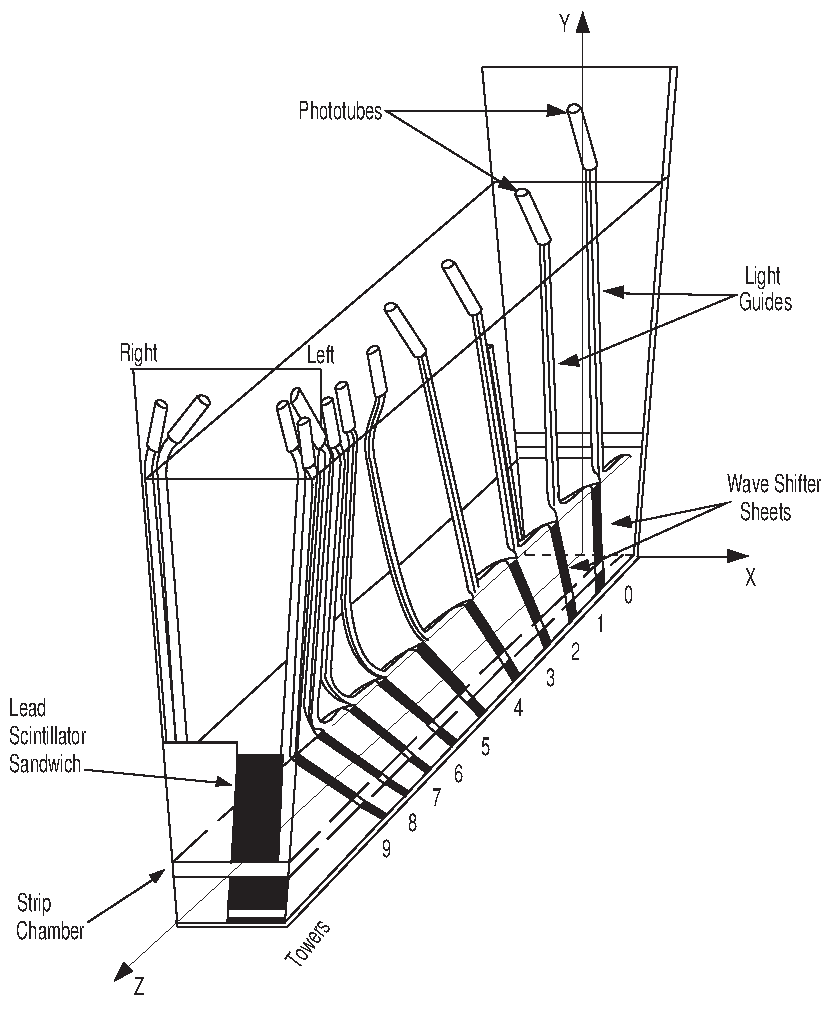
\includegraphics[scale=0.6,keepaspectratio=true]{./cdf_cem_wedge.pdf}
 % cdf_cem_wedge.pdf: 396x486 pixel, 72dpi, 13.97x17.15 cm, bb=0 0 396 486
 \caption{Schematic drawing of a single central calorimeter wedge.}
 \label{fig:CEMwedge}
\end{figure}


\begin{figure}[p]
 \centering
 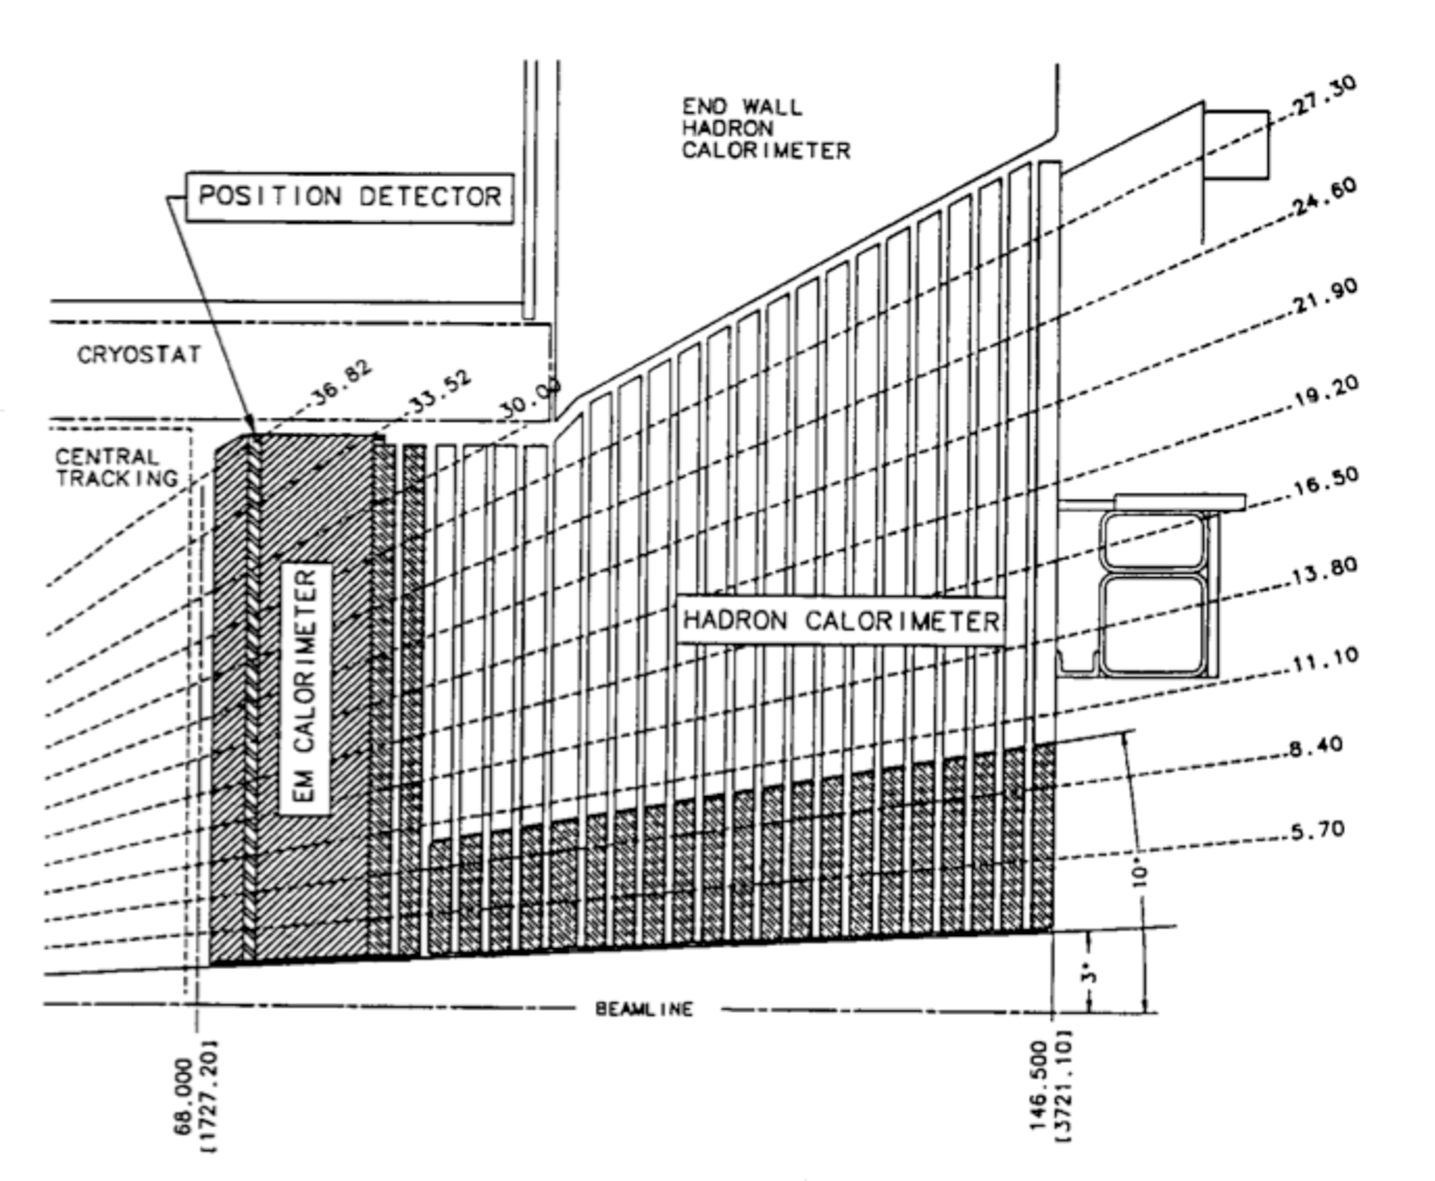
\includegraphics[scale=0.5,keepaspectratio=true]{./plugCalSchem.pdf}
 % plugCalSchem.pdf: 689x567 pixel, 72dpi, 24.31x20.00 cm, bb=0 0 689 567
 \caption{Diagram of a plug calorimeter wedge.}
 \label{fig:PlugCalWedge}
\end{figure}

\vspace{-0.015\textheight}
The central electromagnetic calorimeter (CEM) (Fig.~\ref{fig:CEMwedge}) has an energy resolution of $\sigma(\et)/\et = 13.5\%/\sqrt{\et} \pm 2\%$ and the plug electromagnetic calorimeter (PEM) (Fig.~\ref{fig:PlugCalWedge}) has an energy resolution of $\sigma(\et)/\et = 16.0\%/\sqrt{\et} \pm 2\%$ for an electron. The central hadron calorimeter (CHA) and plug hadron calorimeter (PHA) energy resolution, as measured with pions, is $50\%\sqrt{E} \pm 3\%$ and $80\%\sqrt{E} \pm 5\%$, respectively \cite{pap:PlugCal}. A summary of the detector parameters is shown in Table~\ref{tab:Calo_parameters}.

\begin{table}[p]
\caption{Calorimeter parameters, thicknesses of active and passive materials, and energy resolutions.}
\label{tab:Calo_parameters}
\centering
\begin{tabular}{ccccc}
\hline
 & \BUbf{CEM} & \BUbf{PEM} & \BUbf{CHA} & \BUbf{PHA}\\
\hline
Thickness & 19~$X_{0}$, 1$\lambda$ & 21~$X_{0}$, 1$\lambda$ & 4.5$\lambda$ & 7$\lambda$ \\
Absorber & 0.6~$X_{0}$ & 0.8~$X_{0}$ & 25-50~mm & 50~mm \\
Scintillator & 5~mm & 4.5~mm & 10~mm & 6~mm \\
Resolution & $\frac{13.5\%}{\sqrt{E_{T}}} \pm 2\%$ & $\frac{16.0\%}{\sqrt{E_{T}}} \pm 2\%$ & $\frac{50\%}{\sqrt{E}} \pm 3\%$ & $\frac{80\%}{\sqrt{E}} \pm 5\%$\\
\hline
\end{tabular}
\end{table}

\subsection{Shower Maximum Detector}\label{sec:CES}
The Central Shower Maximum (CES)\glossary{name={CES}, description={Shower Maximum Detector}} detector is located at 7 radiation lengths inside the CEM (Fig.~\ref{fig:CEMwedge}) and provides measurements to determine the position and development of the transverse shower. A simulation of the shower development is shown in Fig.~\ref{fig:ElecCascadeInIron}. By measuring the charge deposition on the set of copper \newterm{strips} lying in the $z$-direction and \newterm{wires} lying orthogonal to strips (Fig.~\ref{fig:CESchamber}), it measures the azimuthal angle and $z$ position of the cluster. The position resolution for a 50~GeV electron is about 2~mm in each direction. The profile of the particle's shower measured by the CES and Plug Shower Maximum (PES) is used to discriminate photons from $\pi^{0}\to\gamma\gamma$ and from electrons. The detector parameters are shown in Table~\ref{tab:CESParamerters}.

\begin{figure}[hbtm]
 \centering
 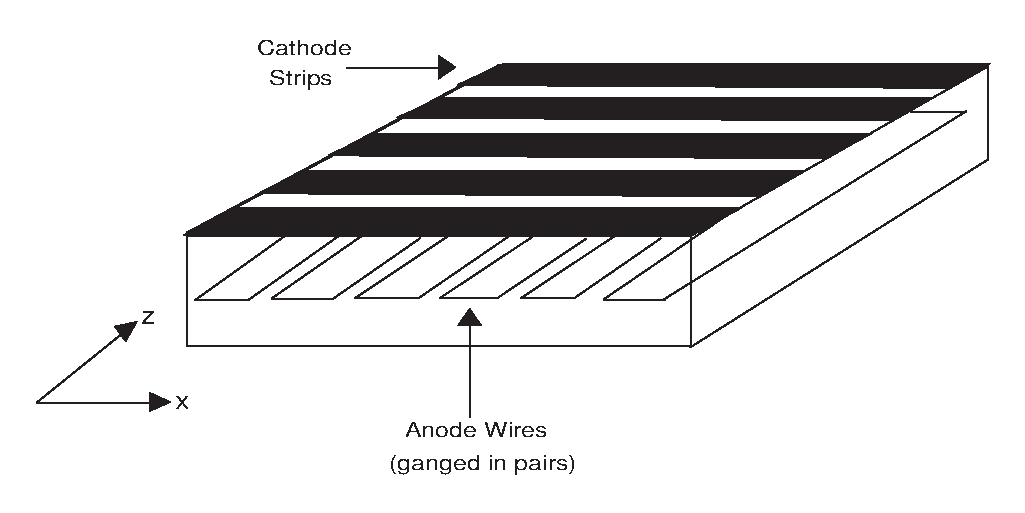
\includegraphics[scale=0.89, keepaspectratio=true]{./ces_chamber.pdf}
 % ces_chamber.pdf: 492x246 pixel, 72dpi, 17.36x8.68 cm, bb=0 0 492 246
 \caption{CES wire and strip chamber.}
 \label{fig:CESchamber}
\end{figure}

\begin{table}[p]
\caption{Shower maximum detector parameters~\cite{pap:CDFCemCalorimeter}.}
\label{tab:CESParamerters}
\centering
\begin{tabular} {cc}
\hline
\BUbf{Parameter} & \BUbf{Value}\\
\hline
Radius from the beam line & 183.9 cm\\[1ex]
\textsc{Wire Channels (64)} & \\
Section 1 & 121.2 cm from the 90\degree edge\\
Wires & 32 $\times$ 1.45484 cm\\
Section 2 & 121.2--239.6 cm from the 90\degree edge\\
Wires & 32 $\times$ 1.45484 cm\\[1ex]
\textsc{Strip Channels (128)} & \\
Section 1 & 6.2--121.2 cm from the 90\degree edge\\
Strips & 69 $\times$ 1.67 cm\\
Section 2 & 121.2--239.6 cm from the 90\degree edge\\
Strips & 59 $\times$ 2.01 cm\\[2ex]
\multirow{3}{*}{\textsc{Total Thickness}} & 0.75 in.\\
& 0.069 radiation lengths\\
& 0.022 absorption lengths\\[2ex]
\textsc{Gas} 	& 95\%/5\% Ar/CO$_{2}$\\
\hline
\end{tabular}
\end{table}

\subsection{Muon Systems}\label{muon_system}
Often the energetic muons produced in collisions escape the CDF detector due to their high penetration power, leaving very little or no energy in the calorimeter. They do not generate a shower when they pass through the detector. The CDF muon detectors are stacked gaseous drift chambers. They form the outermost layer of subdetectors. They are designed to identify the ionization energy signature, and hits in chambers are combined to identify a track that indicates the presence of a muon in the event.

\subsection{Calorimeter Timing System}\label{EMTiming}
The timing readout for the electromagnetic calorimeters was installed as part of an upgrade for Run II. The system, known as \newterm{EM Timing}, has a resolution of less than a nanosecond and covers the central ($|\eta| < 1.1$) and plug ($1.1 < |\eta| < 2.1$) portions of the calorimeter \cite{pap:EMtiming}. A schematic diagram of the electronics of the system is shown in Fig.~\ref{fig:EMtimingSchematic}. The design of the EM Timing system is optimized for high-energy photons. It records the time of arrival of the particles that deposit large amounts of energy in the electromagnetic calorimeter. With this information it is possible to verify that all photons (or other energy) are from the primary collision, and also to reject or estimate the rate of cosmic-ray and beam-related backgrounds (see Section \ref{noncollision_backgrounds}). An overview of the EM Timing system parameters is listed in Table~\ref{tab:EMTimingPerformance}.

\begin{figure}[htb!]
 \centering
 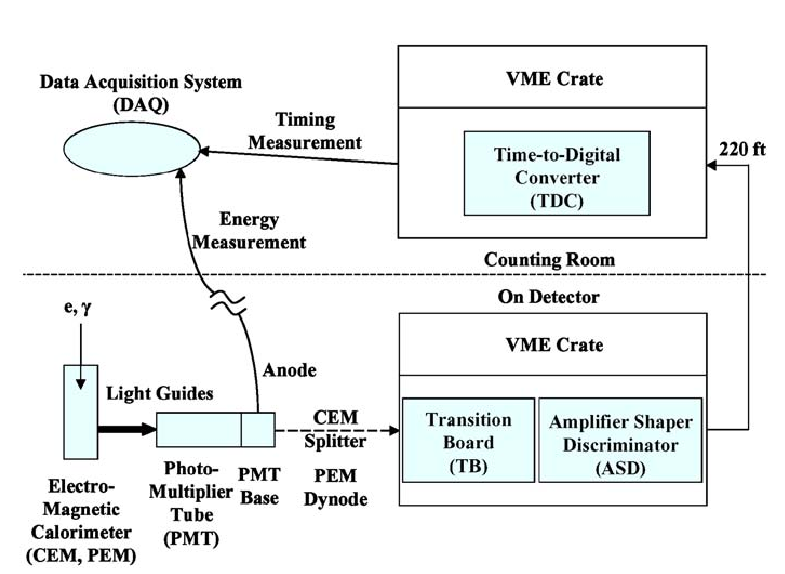
\includegraphics[scale=0.5,keepaspectratio=true]{./EMtimingSchematic.png}
 % EMtimingSchematic.png: 785x574 pixel, 96dpi, 20.77x15.19 cm, bb=0 0 589 430
 \caption{A schematic diagram of the EM Timing system hardware on the CDF detector.}
 \label{fig:EMtimingSchematic}
\end{figure}

\begin{table}
\caption{Overview of the EM Timing system hardware and performance.}
\label{tab:EMTimingPerformance}
\centering
\begin{tabular}{lcc}
\hline
& \BUbf{CEM} & \BUbf{PEM}\\
\hline
Coverage & $|\eta|<1.1$ & $1.1<|\eta|<2.1$\\
Physical tower segmentation & $\Delta\phi=15\degree$, & $\Delta\phi=7.5\degree$,\\
& $\Delta \eta \approx 0.1 $ & $\Delta \eta \approx 0.1$\\[1ex]
Energy threshold & $3.8\pm0.3$~GeV & $1.9\pm0.1$~GeV\\
Timing resolution & $600\pm10$~ps & $610\pm10$~ps\\
\hline
\end{tabular}
\end{table}


\subsection{Extremely Fast Tracker (XFT)}
The eXtremely Fast Tracker (XFT) \cite{pap:XFT} is a vital part of the CDF trigger system. It is a trigger track processor that identifies charged tracks in the COT. This track information is made available to both Level 1 and Level 2 trigger decisions. The XFT is fully pipelined and provides track information for every event. The tracks are not fitted, but compared to predetermined patterns (or \newterm{roads}) derived using Monte Carlo methods. It is designed to measure tracks with momenta as low as \ptg{1.5}, to have high momentum and position resolution, and to minimize the fraction of tracks that are not associated with a real charged particle (\newterm{fake tracks}).

The XFT algorithm uses the hit information from the 4 axial superlayers of the COT. A charged track passing through an axial layer will generate a characteristic hit pattern in a 12-wire COT cell and will have a characteristic timing. The hit information in a superlayer is used by the Finders to search for track segments in the axial layers. Then the Linker will search and match track segments in the 4 superlayers to a track originated from the primary collision point. The Linker is able to search for tracks in 4/4 as well as 3/4 matches among the segments in the 4 layers.

As seen in Fig.~\ref{fig:XFTStructure}, the COT wire signals (pulses) are digitized by the Time-to-Digital Converters (TDC). The TDCs output the arrival time of the pulses (or time indices). The XTC mezzanine cards, mounted on the TDCs, use these time indices to categorize the hits on the COT wires into \newterm{prompt} ($<44$~ns) or \newterm{delayed} ($>44$~ns). The XTC sends the information to the Finder for processing.

\begin{figure}[htbm!]
 \centering
 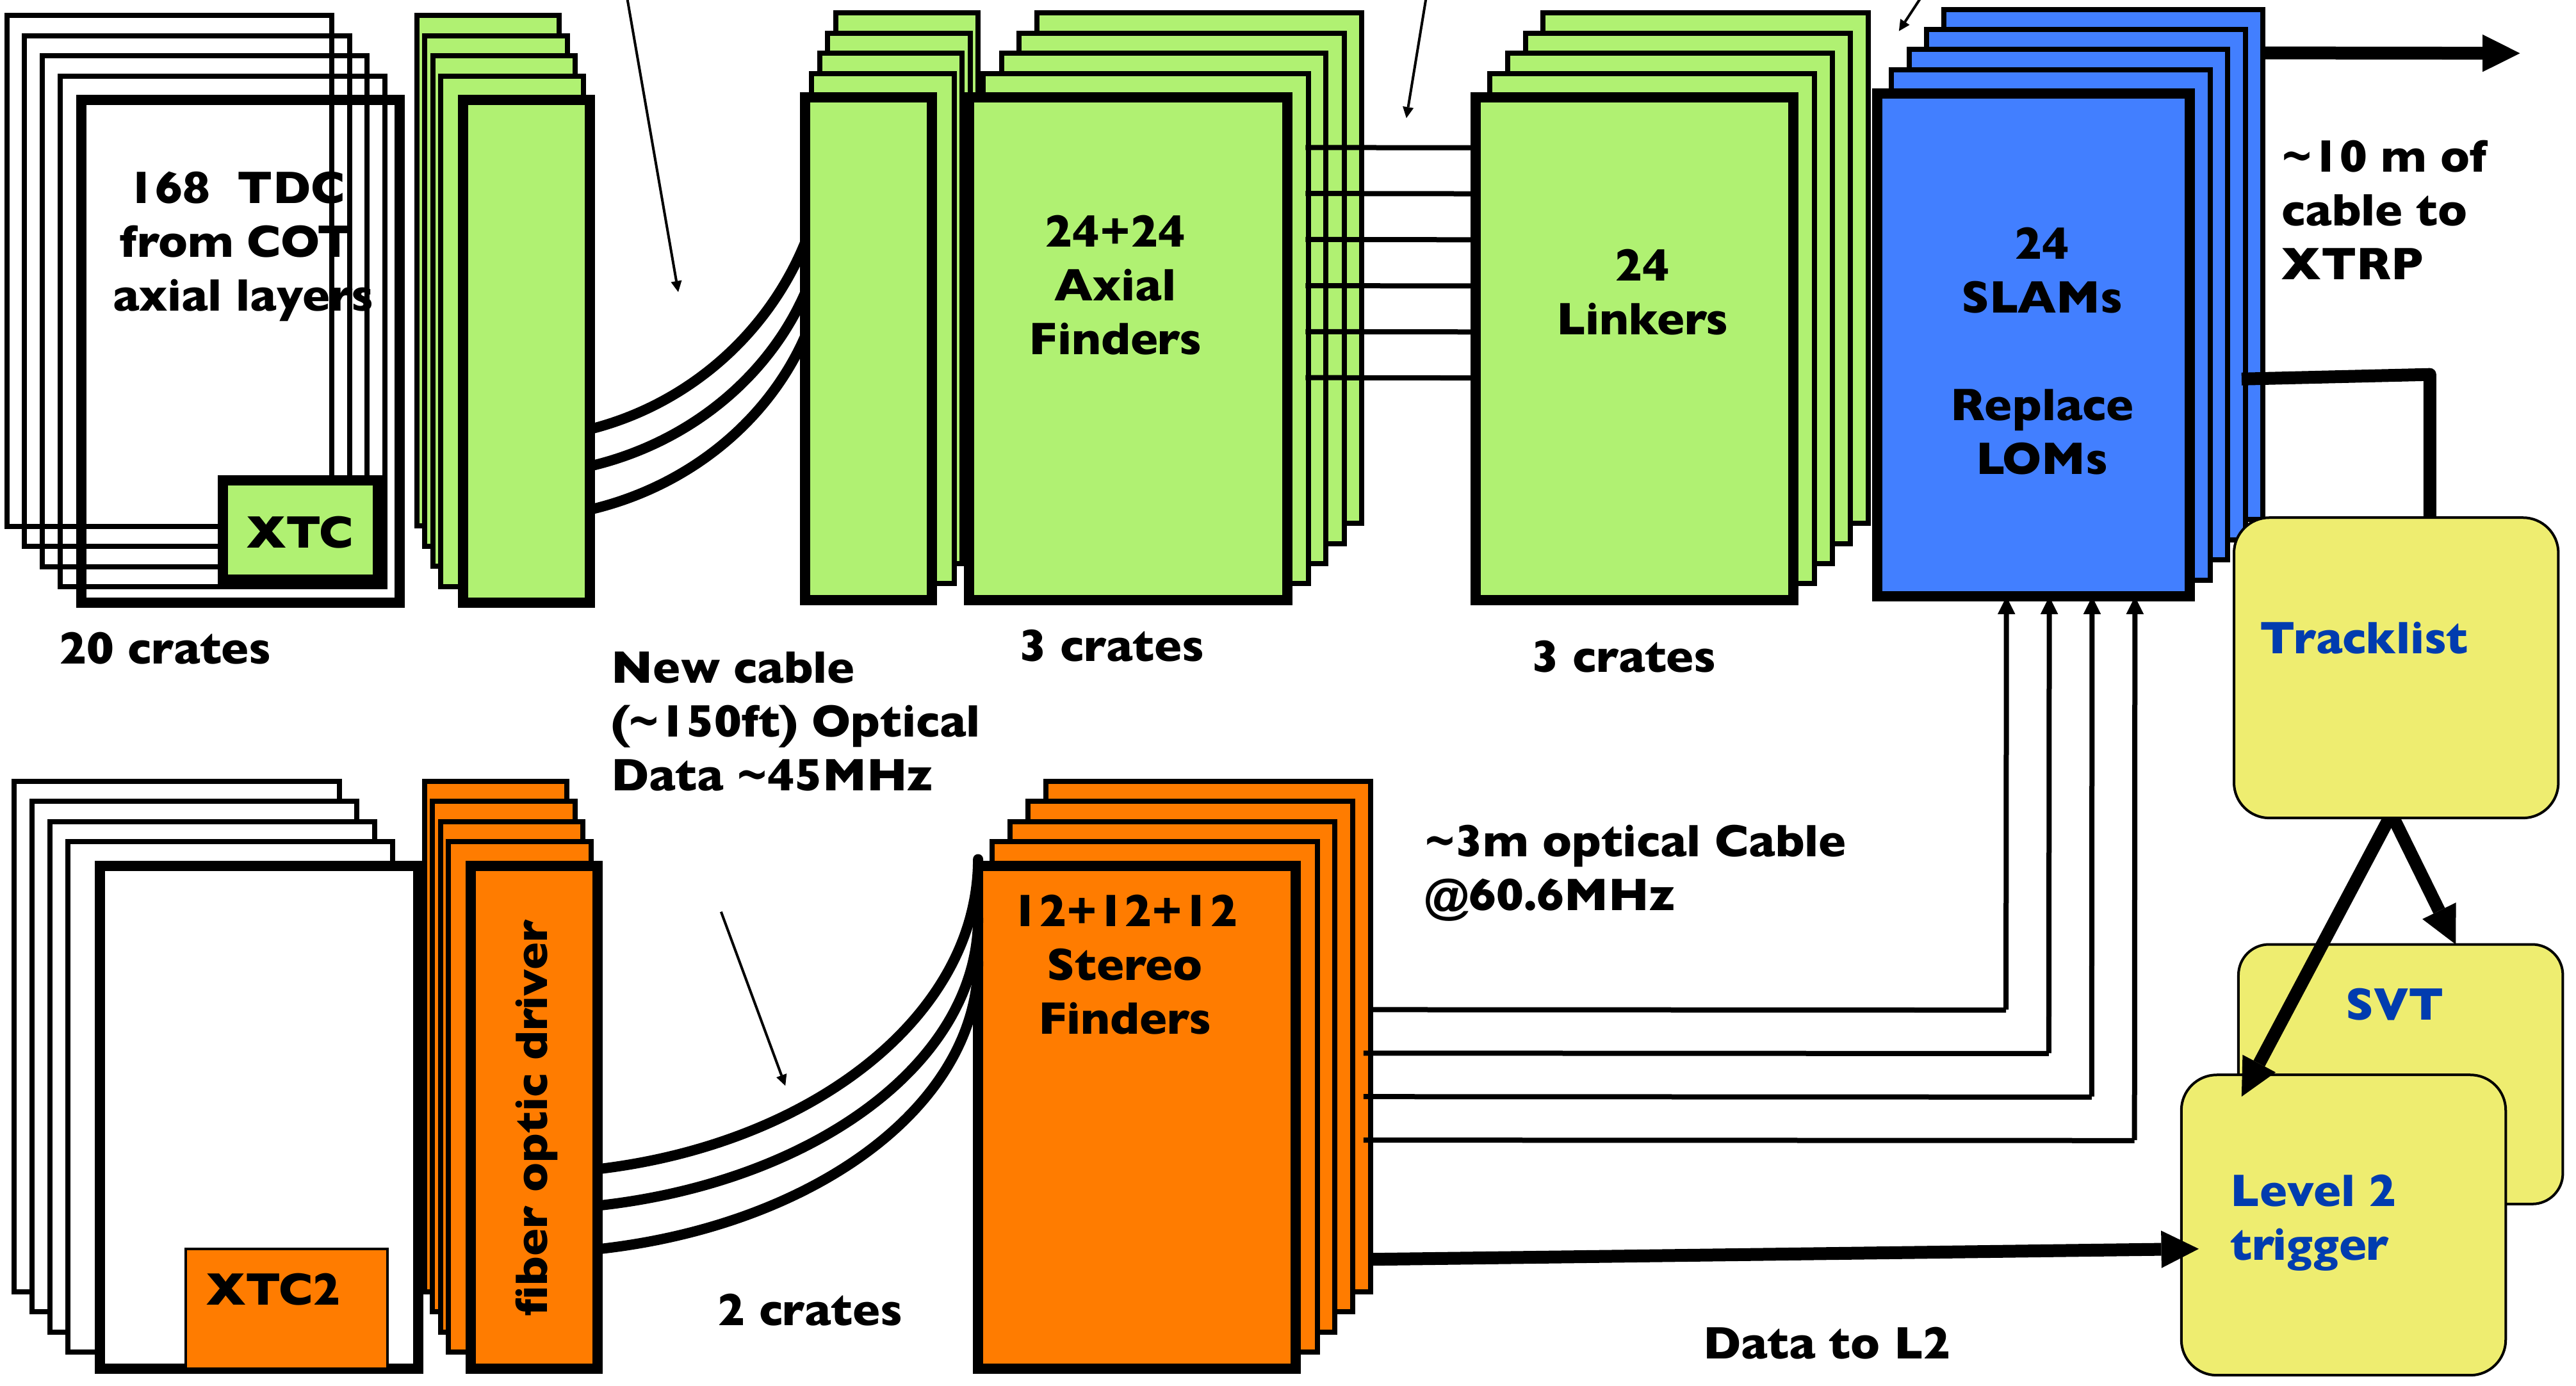
\includegraphics[scale=0.14,keepaspectratio=true]{./XFTStructure.png}
 % XFTStructure.png: 774x470 pixel, 96dpi, 20.48x12.43 cm, bb=0 0 580 352
 \caption{Design of the XFT system. The upgrade added the stereo superlayer information to the existing axial system to enhance the track purity. The new fiber optic data path via XTC2$\to$Stereo Finder is merged with the axial system by the Stereo Linker Association Module, which associates the axial track segments with stereo track segments. The track information is then passed onto Level 2 decision-making and to the vertex detector.}
 \label{fig:XFTStructure}
\end{figure}
\vspace{-0.01\textheight}

The XFT was upgraded in summer of 2006 to handle the increased instantaneous luminosity. This was necessary as the higher luminosity increases the COT occupancy and produces many more fake tracks, which leads to a higher trigger rate. To handle this, the existing axial system was kept intact and the Stereo Finder system was added. The hit information from the 4 stereo superlayers is used by the Stereo Finder system to find track segments and confirm the association of those segments with the axial track segments. This also allows the measurement of the track's $z$ direction to match with the calorimeter or muon chambers.

The boxes colored in orange and blue in Fig.~\ref{fig:XFTStructure} indicate the new components. The new XTCs (called XTC-2) are able to classify hits into 6 programmable time windows. The Stereo Finder uses this information to identify track segments in the stereo layers. The Stereo Linker Association Module (SLAM) associates stereo track segments with the axial tracks. The performance of the XFT system is summarized in Table~\ref{tab:XFTperformance}.

\begin{table}
\caption{Performance of the XFT system as measured by data.}
\label{tab:XFTperformance}
\centering
\begin{tabular}{lc}
\hline
\BUbf{Parameter} & \BUbf{Value}\\
\hline
Efficiency & 96\% \\
Percentage Fakes & 3\% \\
Momentum Threshold & 1.5~\epUnits \\
Momentum Resolution & 1.7\%/\epUnits \\
Angular Resolution & 5.5~mR\\
\hline
\end{tabular}

\end{table}

The XTC and Finder electronics are designed with Field Programmable Gate Arrays (FPGA), which allow one to program custom logic designs into the electronics. The author performed preliminary testing of the XTC-2 cards and Finder boards and has implemented software packages to reprogram the XTC-2s and Finders. The conventional Finder FPGA reprogramming was sequential. Given that the Axial Finder boards require the loading of 4 logic designs, and each design requires about 20~s to download, reprogramming 48 of them took a considerable amount of time.

\begin{sidewaysfigure}[p]
 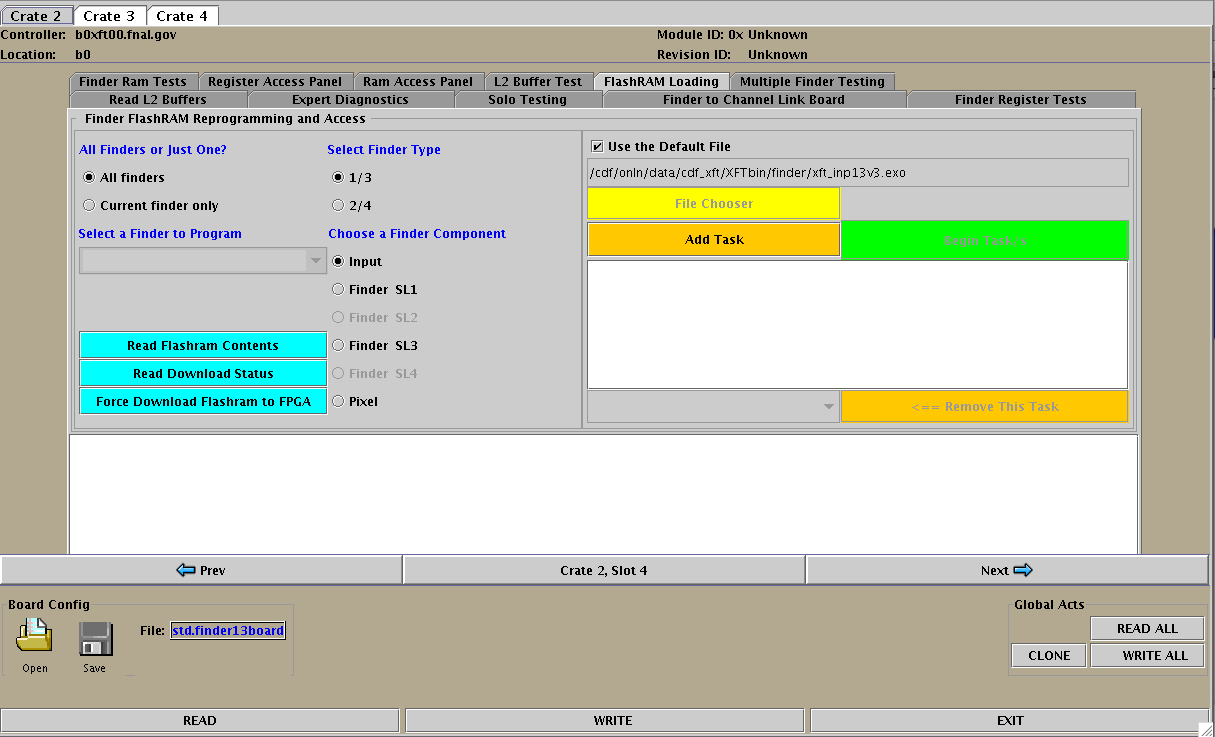
\includegraphics[scale=0.5,keepaspectratio=true]{./FlashRAMprogram.png}
 % FlashRAMprogram.png: 1215x737 pixel, 72dpi, 42.86x26.00 cm, bb=0 0 1215 737
 \caption{Graphical interface of the Finder Flash RAM program.}
 \label{fig:FlashRAMprogramming}
\end{sidewaysfigure}

This shortcoming was overcome by introducing a novel parallel programming technique known as \newterm{multithreading}. In general, multithreading forks a computer program into two or more concurrently running tasks or processes with the aid of techniques like time-division multiplexing to share the CPU time effectively among tasks. With this technique, all 48 of the Finder boards can be loaded with a specific design at once. The program is capable of job queuing to further reduce the downtime and speed up the Finder reprogramming. The interface of the program is shown in Fig.~\ref{fig:FlashRAMprogramming}. In addition, it can program a single Finder board with a specific software design and it can check the download status and the loaded software version on the boards.

Furthermore, the author developed software to reprogram XTC-2 cards from the unix command line. This is especially useful when working remotely with slower network connections. Also, the old \newterm{cratemap} program was updated to suit the upgrade system. The cratemap program scans crates holding the TDCs, Finders, etc. and provides information about the boards loaded into crates and their software versions and other information for diagnostics.

\subsection{Track Extrapolation Module (XTRP)}
The Track Extrapolation Module, XTRP for short, is part of the L1 trigger system driven by the information from the XFT. The XTRP distributes information derived from the tracks to make Level 1 and Level 2 trigger decisions. It performs three main tasks as shown it Fig.~\ref{fig:XTRPdataflow}. It extrapolates tracks to the central muon system and sends the information to the Level 1 MUON trigger. Similarly, information about tracks extrapolated to the central calorimeter is sent to L1 CAL trigger. Also, it selects tracks above a given \pt threshold and uses \pt and $\phi$ information to define the Level 1 TRACK trigger. Finally, the track information is passed on to Level 2 processing and the SVX upon a Level 1 accept.

\begin{figure}[htb!]
 \centering
 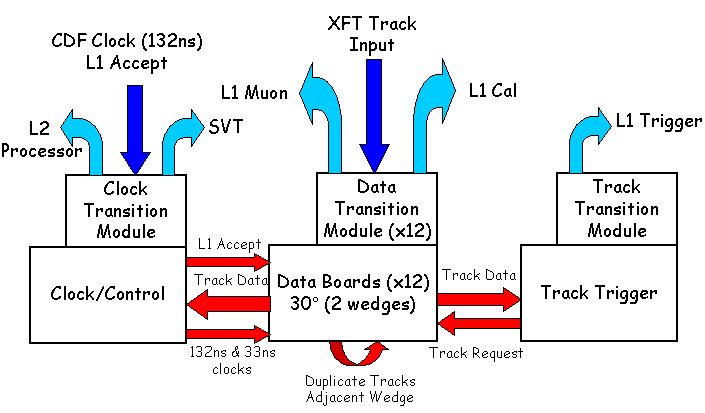
\includegraphics[scale=0.6]{./XTRP_dataflow.png}
 % XTRP_dataflow.gif: 720x540 pixel, 72dpi, 25.40x19.05 cm, bb=0 0 720 540
 \caption{Dataflow of the XTRP system.}
 \label{fig:XTRPdataflow}
\end{figure}


\subsection{Triggering}\label{triggering}
The Tevatron physics objective is to produce and study rare events. With a beam crossing interval of 396~ns, about a million events are generated every second. With the total inelastic cross section of about 60~mb, extracting signals of interest in an efficient way is an enormous challenge. Also, system limitations allow the recording of only a relatively small number of events per second. The solution is a \newterm{trigger} which will flag an event that satisfies a certain set of predefined kinematic thresholds (\textit{e.g.} transverse track momentum, calorimeter energy) and objects (\textit{e.g.} electron, muon, jet). A trigger is designed with a specific physics motivation and implemented after an extensive study. A collection of such individual triggers form a \newterm{trigger table}. The CDF trigger rejection is about 25000.

An efficient trigger requires fast object reconstruction and matching of tracks with the objects. The trigger matches COT tracks with EM calorimeter showers, muon chamber stubs, and silicon detector data in making a decision to save an event for physics analysis.

The CDF has a three-tier trigger system that is fully pipelined and hence deadtimeless (See Figs.~\ref{fig:TriggerSystemDetParts} and ~\ref{fig:TriggerSystemSchematic}). It is capable of dynamically limiting the acceptance of certain high rate processes as the luminosity changes. The \newterm{Level~1} trigger system is entirely hardware based, optimized for a quick decision. It forms trigger primitives by reading out a subset of detector components (like the tracking systems and calorimeters) and makes the initial decision to process the event further. Level~1 makes its decision to further process the event based on the information from the XFT, calorimeter, and muon data as seen in Fig.~\ref{fig:TriggerSystemDetParts}.

\begin{figure}[p]
\begin{centering}
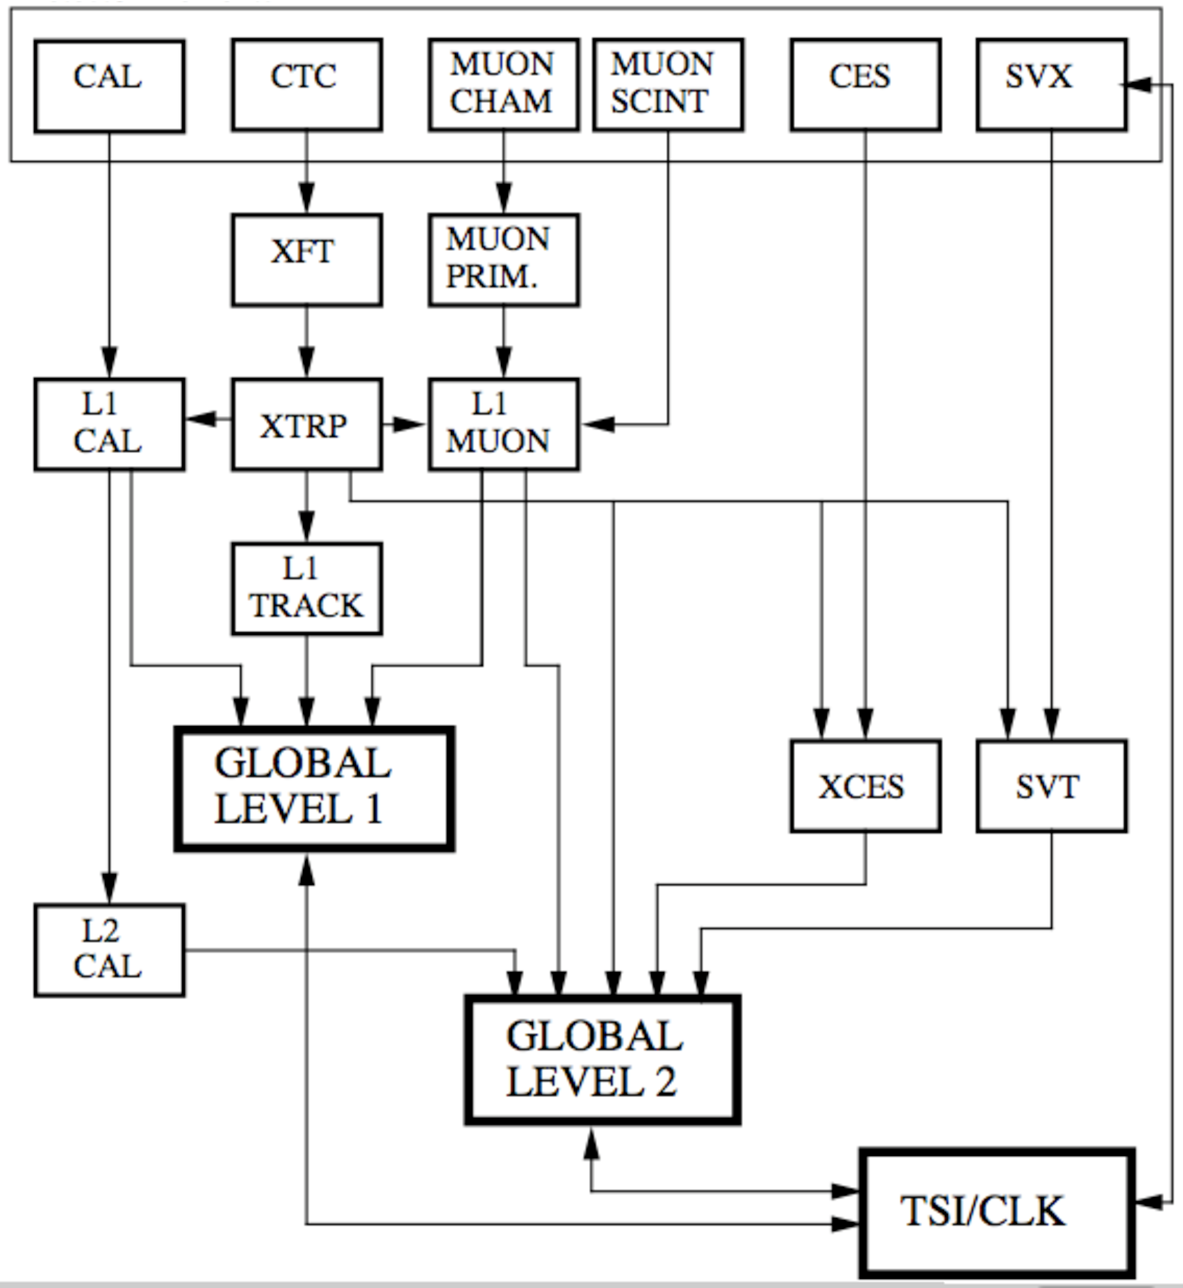
\includegraphics[scale=0.7]{CDFTriggerSystem_DetParts.pdf}
\caption{Block diagram of the CDF three-level trigger system. This shows the detector information available at each decision level.}%Some detector components readout time is significantly large and is not used in initial decision making.}
\label{fig:TriggerSystemDetParts}
\end{centering}
\end{figure}

\begin{figure}[p]
\begin{centering}
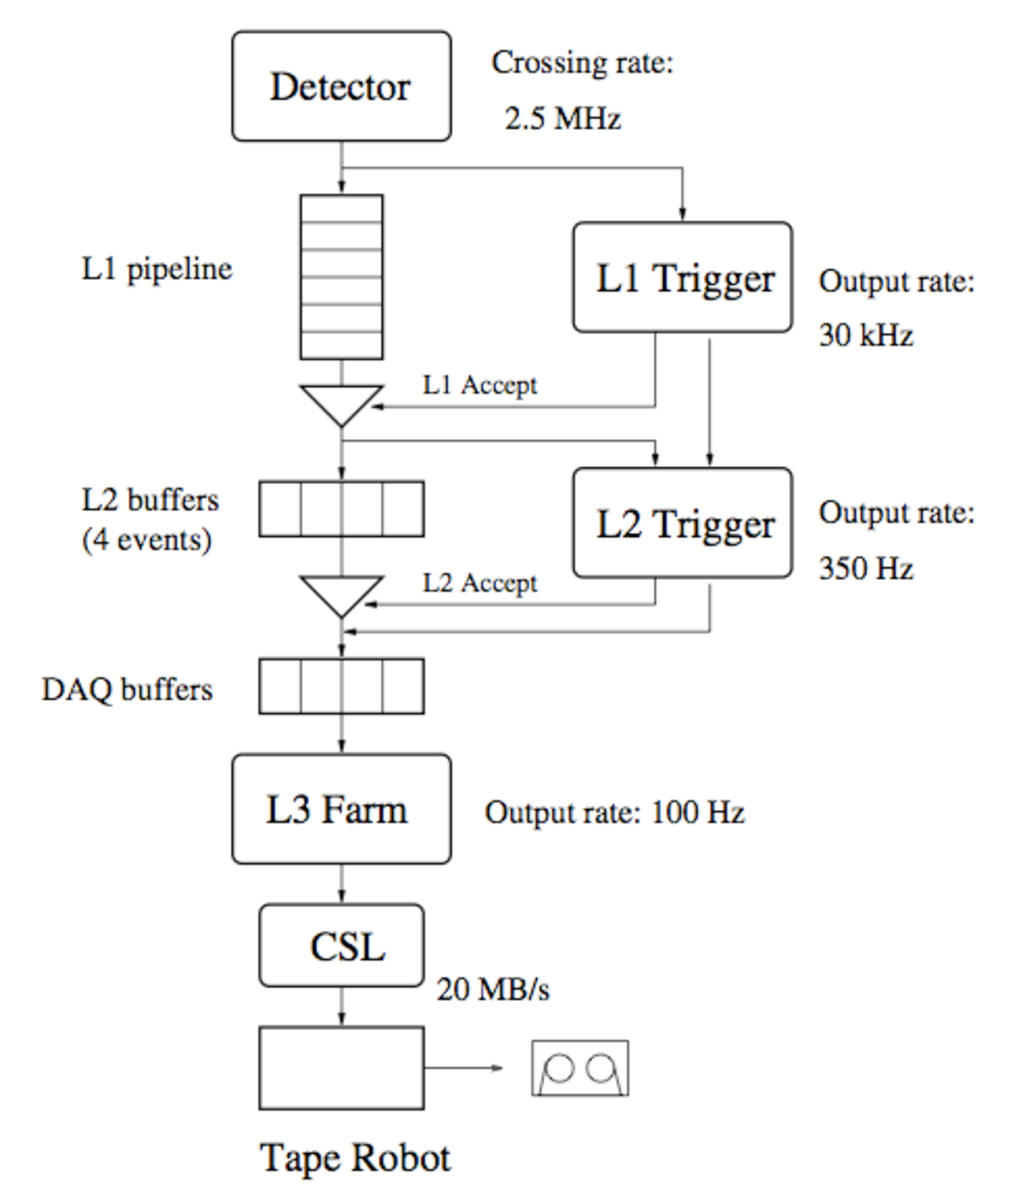
\includegraphics[scale=0.8]{CDFTriggerSystem_Scehmatic.pdf}
\caption{Dataflow of CDF \newterm{deadtimeless} trigger system. Optimized by fully pipelining the system to match the physics event rate to the data acquisition rate.}
\label{fig:TriggerSystemSchematic}
\end{centering}
\end{figure}


The \newterm{Level 2} trigger is a combination of hardware and software and the output rate is lower. It also has more information available to make a more accurate decision. \newterm{Level 3} is entirely software-based and makes its final decision by completely reconstructing the event. The final output rate to tape is about 100~Hz. Overall, the trigger system rejects 99.99\% of events produced.


%Acceptance is defined as the probability that the generated (Monte Carlo) particles pass transverse energy (\et) , detector $\eta$ and other geometric cuts such as the azimuthal separation between objects. The efficiency is probability to survive all other sources of event losses.The distinction is that the acceptance can be calculated by anyone with access to a MC generator such as PYTHIA. The efficiency requires a detailed simulation of the detector with additional corrections and cross checks from data samples.


\subsection{Run Number, Run Section, and Run Period}
Each continuous data collection period is identified by a integer called a \newterm{run number}. To prevent data loss during a \newterm{run}, data are subdivided into about 15~sec periods called \newterm{run sections}. The importance of this is, for example, if a certain detector component is recognized to be at fault during a run, but not necessarily throughout the whole run, by identifying the time the fault occurred, data collected until that point can be recovered. A run period is about 2--3 months worth of data-taking time and depends on many factors like the amount of data collected and the detector operation status.

\subsection{Good Run List}\label{sec:GoodRun}
For some analyses, not all the information from the whole detector is needed. Information from certain subdetector components may not be crucial and may be omitted. An analysis expert will make a list of run numbers that had the required detector components running while the data of interest was collected. This list of run numbers is called a \newterm{good run list}. For photon analyses, it is necessary for COT, CES/PES, and calorimeters to be marked good. This study uses the good run list labeled by \goodrunfile.

